\documentclass[
12pt, % Main document font size
a4paper, % Paper type, use 'letterpaper' for US Letter paper
oneside,
% One page layout (no page indentation)
%twoside, % Two page layout (page indentation for binding and different headers)
%hidelinks, % Hide links like hyperref
%headinclude,footinclude, % Extra spacing for the header and footer
%BCOR5mm, % Binding correction
]{article}



\setlength{\parindent}{5pt} %Modifica la dimensione dell'indentazione dei paragrafi



%%%%% Packages
%\usepackage [english]{babel}
\usepackage [italian]{babel}

\usepackage{enumitem} % migliori enumerate, ad esempio \begin{enumerate}[label=\Alph*]

%per far chiudere e aprire " "
%\usepackage [autostyle, english = american]{csquotes}
%\MakeOuterQuote{"}

\usepackage{hyphenat}
\begin{hyphenrules}{english}
\hyphenation{Fortran}
\hyphenation{spa-sti-ci-ty} 
\end{hyphenrules}

\usepackage[section]{placeins} %Also one can consider the placeins package and the \FloatBarrier command that prevents figures from floating any further. If figures are supposed to remain in the section, one can load

\usepackage{tabularx} %advance tables, like wrap text inside cell
\usepackage{longtable}

\usepackage{graphicx}
%\usepackage{subfig}
\usepackage{xcolor} %Colori Aggiuntiv
\usepackage[colorlinks = true,
	linkcolor = teal,
	urlcolor  = blue,
	citecolor = teal,
	anchorcolor = blue]{hyperref} %Hyperref
	
% listings for code	
\usepackage{listings}
\usepackage{color}
\definecolor{dkgreen}{rgb}{0,0.8,0}
\definecolor{gray}{rgb}{0.5,0.5,0.5}
\definecolor{mauve}{rgb}{0.58,0,0.82}

\lstset{frame=shadowbox,
  language=Matlab,
  aboveskip=3mm,
  belowskip=3mm,
  showstringspaces=false,
  columns=flexible,
  basicstyle={\small\ttfamily},
  numbers=none,
  numberstyle=\tiny\color{gray},
  keywordstyle=\color{blue},
  commentstyle=\color{dkgreen},
  stringstyle=\color{mauve},
  breaklines=true,
  breakatwhitespace=true,
  tabsize=3
}


\usepackage{url}

%\usepackage{lipsum} %Crea dummy text

\usepackage{amsmath,amssymb,amscd,amsfonts,amsthm} %Roba matematica

%bibliografia
%\usepackage[shortalphabetic,abbrev]{amsrefs}
%\usepackage[author-year, y2k]{amsrefs}
\usepackage[alphabetic]{amsrefs}
\usepackage{mathtools}

\usepackage{physics}

\usepackage{siunitx} %database unita` di misura, \si{ \kg \per \second},  \SI{20}{ \kg \per \second}
\sisetup{
	round-mode          = places,
	round-precision     = 2,
}

\usepackage{gensymb} %simboli extra, come \degree

\usepackage{tikz}
	\usetikzlibrary{shapes,arrows}
	\tikzstyle{block} = [draw, fill=white, rectangle, 
	minimum height=3em, minimum width=6em]
	\tikzstyle{sum} = [draw, fill=white, circle, node distance=1cm]
	\tikzstyle{input} = [coordinate]
	\tikzstyle{output} = [coordinate]
	\tikzstyle{pinstyle} = [pin edge={to-,thin,black}]
	\usepackage{tikzscale}

\usepackage{pgfplots}
	\pgfplotsset{width=7cm,compat=1.14}
	%\pgfplotsset{compat=newest} % Allows to place the legend below plot
	\pgfplotsset{every minor tick/.append style={thin}}  % applies only to minor ticks,
	\usepgfplotslibrary{units} % Allows to enter the units nicely
	%\usepgfplotslibrary{external} 
	%\tikzexternalize
	%\tikzset{external/force remake}
	\pgfkeys{/pgf/number format/.cd,1000 sep={\,}}

\usepackage{afterpage}

\usepackage{comment} % inserisce la funzionalita` \begin{comment}
\usepackage{wrapfig}
\usepackage{vmargin}
\setmarginsrb  {25mm}  % left margin
	{ 5mm}  % top margin
	{25mm}  % right margin
	{15mm}  % bottom margin
	{10mm}  % head height
	{15mm}  % head sep
	{10mm}  % foot height
	{15mm}  % foot sep

% permettono l'uso di subfigures
\usepackage{caption}
\usepackage{subcaption}


%%%%%%%%%%%%%%%%%%%%%%%%%%%%%%%%%%%%%%%%%%%%%%%%%%%%%%%%%%
%%%%% Comandi homebrewed


%% comando per fare matrix con linee verticali. Esempio:
%\[
%\begin{pmatrix}[cc|c]
%  1 & 2 & 3\\
%  4 & 5 & 9
%\end{pmatrix}
%\]
\makeatletter
\renewcommand*\env@matrix[1][*\c@MaxMatrixCols c]{%
  \hskip -\arraycolsep
  \let\@ifnextchar\new@ifnextchar
  \array{#1}}
\makeatother


%% renew comando paragraph per far andare a capo dopo \paragraph
\newcommand{\myparagraph}[1]{\paragraph{#1}\mbox{}\\}

\newcommand{\bs}{\textbackslash}

%% BLANKPAGE
%per creare pagine vuote
\newcommand\blankpage{%
	\null
	\thispagestyle{empty}%
	%\addtocounter{page}{-1}%
	\newpage}

%% RNUM 
% porta in numeri romani il unmero
\newcommand{\RNum}[1]{\uppercase\expandafter{\romannumeral #1\relax}}

%% AT
% Comando per le derivate calcolate nel punto. Esempio: \dv{\text{Im}T(j \omega)}{t} \at[\Big]{\omega = \omega_1}
\newcommand{\at}[2][]{#1|_{#2}}

%% Comando per valori assoluti che scalano
%\DeclarePairedDelimiter\abs{\lvert}{\rvert}%
%\DeclarePairedDelimiter\norm{\lVert}{\rVert}%
% Swap the definition of \abs* and \norm*, so that \abs
% and \norm resizes the size of the brackets, and the 
% starred version does not.
\makeatletter
\let\oldabs\abs
\def\abs{\@ifstar{\oldabs}{\oldabs*}}
%
%\let\oldnorm\norm
%\def\norm{\@ifstar{\oldnorm}{\oldnorm*}}
\makeatother

%% CEILING and FLOOR
\DeclarePairedDelimiter\ceil{\lceil}{\rceil}
\DeclarePairedDelimiter\floor{\lfloor}{\rfloor}

% %% Prova theorem
% \newtheorem{theorem}{Theorem}[section]
% \newtheorem{lemma}[theorem]{Lemma}
% \newtheorem{proposition}[theorem]{Proposition}
% \newtheorem{corollary}[theorem]{Corollary}

% \newenvironment{Proof}[1][Proof]{\begin{trivlist}
% 		\item[\hskip \labelsep {\bfseries #1}]}{\end{trivlist}}
% \newenvironment{definition}[1][Definition]{\begin{trivlist}
% 		\item[\hskip \labelsep {\bfseries #1}]}{\end{trivlist}}
% \newenvironment{example}[1][Example]{\begin{trivlist}
% 		\item[\hskip \labelsep {\bfseries #1}]}{\end{trivlist}}
% \newenvironment{remark}[1][Remark]{\begin{trivlist}
% 		\item[\hskip \labelsep {\bfseries #1}]}{\end{trivlist}}

%\newcommand{\qed}{\nobreak \ifvmode \relax \else
%	\ifdim\lastskip<1.5em \hskip-\lastskip
%	\hskip1.5em plus0em minus0.5em \fi \nobreak
%	\vrule height0.75em width0.5em depth0.25em\fi}

%% \xoverline
% simile a \bar ma copre tutta il width della lettera
\makeatletter
\newsavebox\myboxA
\newsavebox\myboxB
\newlength\mylenA

\newcommand*\xoverline[2][0.75]{%
    \sbox{\myboxA}{$\m@th#2$}%
    \setbox\myboxB\null% Phantom box
    \ht\myboxB=\ht\myboxA%
    \dp\myboxB=\dp\myboxA%
    \wd\myboxB=#1\wd\myboxA% Scale phantom
    \sbox\myboxB{$\m@th\overline{\copy\myboxB}$}%  Overlined phantom
    \setlength\mylenA{\the\wd\myboxA}%   calc width diff
    \addtolength\mylenA{-\the\wd\myboxB}%
    \ifdim\wd\myboxB<\wd\myboxA%
       \rlap{\hskip 0.5\mylenA\usebox\myboxB}{\usebox\myboxA}%
    \else
        \hskip -0.5\mylenA\rlap{\usebox\myboxA}{\hskip 0.5\mylenA\usebox\myboxB}%
    \fi}
\makeatother

%%



\graphicspath{{./figs/}}

\begin{document}
	
\begin{titlepage}
	\centering
	\vspace*{0.0 cm}
	
\includegraphics[height=.2\textheight]{figs/cherubino_pant541.pdf}\\[0.5 cm]			% University Logo
	\textsc{\Large Universit\`a di Pisa }\\[0.5 cm]							% University Name
	\textsc{\large Laurea Magistrale \\ 
		\vspace{2mm} in Ingegneria Robotica e dell'Automazione}\\[0.5 cm]
	\textsc{Progetto di Sistemi di Guida e Navigazione}\\[0.25 cm]	
	
	\rule{\linewidth}{0.2 mm} \\[0.4 cm]
	{ \Large{\textbf{Navigazione attraverso AMCL e sistema UWB}}}\\
	\rule{\linewidth}{0.2 mm} \\[0.5 cm]
	%\vspace*{0.5 cm}
	
	\includegraphics[height=0.3\textheight]{charlie_vista_assonometrica.pdf}\\	
	\vspace{1 cm}
	
	
	\begin{minipage}{0.48\textwidth}
		\begin{flushleft}
			\textit{Autori:}\\
			Alessia Biondi\\
			Francesco Petracci
			
			
		\end{flushleft}
	\end{minipage}~
	\begin{minipage}{0.48\textwidth}
		\begin{flushright}    
			\textit{Professore:}\\		
			Lorenzo Pollini\\
		\end{flushright}
	\end{minipage}\\[2 cm]

	
\end{titlepage}
\newpage

% pagina vuota e indice
\newpage\null\thispagestyle{empty}\newpage
\newpage
\pagenumbering{arabic}
\setcounter{page}{1}
\tableofcontents
\newpage

%%%%%%%%%%%%%%%%%%%%%%%%%%%%%% 
% TO DO
%	1.
%	2.
%	3.
%
%
%%%%%%


%%%%%%%%%%%%%%%%%%%%%%%%%%%%%%%%%%%%%%%%%%%%%%%%%%%%%%%%%%%%%%%%%%%%%%%%%%%%%%%%%%%%%%%%%%%%%%%%%%%%%%
% introduzione
\section*{Introduzione}
L'obiettivo di questo progetto \`e stato quello di migliorare lo stato del veicolo, partendo dal risolvere le molte problematiche accumulatesi nel passaggio di 
testimone tra i gruppi precedenti.
Lo scopo principale dell'intero sistema, composto dal veicolo affiancato da una serie di sensori, \`e quello di riuscire a localizzarsi all'interno di una mappa 
preacquisita e di navigare al suo interno.
La posizione \`e ottenuta seguendo due metodologie tra loro complementari: da una parte viene sfruttato un lidar montato sul corpo del veicolo, che permette di 
avere buoni risultati in ambienti chiusi in cui siano presenti pareti e confini ben precisi, dall'altra si appoggia ad un sistema Ultra Wide Band (UWB), che ha 
invece performance migliori in ambienti esterni e privi di ostacoli, sui quali il segnale potrebbe avere interferenze dovute a scattering.
\`E importante sottolineare fin da subito che, tramite il lidar, non viene effettuata una SLAM vera e propria bens\`i uno Scan Matching: infatti, l'algoritmo di 
localizzazione in condizioni nominali prende come posa del veicolo quella ottenuta dallo scan matcher. 
Quest'ultima viene quindi periodicamente confrontata con quella misurata dal sistema UWB, la quale non rappresenta, in condizioni standard, un indice della posizione 
del veicolo. Solo nel momento in cui i due valori, restituiti da Lidar e UWB, differiscono di molto, allora l'ultima posa ottenuta dalle antenne viene assegnata al 
veicolo stesso come sua posa attuale.
In questo modo si ottiene un sistema robusto alla perdita del lidar, che pu\`o verificarsi a seguito di una rottura del sensore o nel momento in cui sono esplorati 
ambienti dove le condizioni non permettono di avere misure affidabili.

\subsection*{Funzionamento in due parole}
Molto sinteticamente andiamo a descrivere il funzionamento di Charlie. 
In primis viene utilizzato il pacchetto hector-slam allo scopo di pre-acquisire e realizzare una mappa dell'ambiente nel quale il veicolo dovrà poi muoversi. 
Solo in un secondo momento, utilizzando questa mappa, avrà luogo la fase di moto, durante la quale il sistema riesce a localizzarsi nell'ambiente attraverso 
l'algoritmo Adaptive Monte Carlo Localization, nel quale ha luogo il confronto tra le misure acquisite dal lidar e le feature della mappa stessa. 

Dato che questo algoritmo può convergere su una posa del veicolo non corretta a causa, per esempio, di ambiguità  tra simmetrie della mappa 
il sistema UWB fa sì che venga reinizializzato l'algoritmo AMCL. 
In questo utilizzo quindi il sistema UWB serve solamente come check.

\subsection*{Come ottenere codice}
Il codice sviluppato è disponibile nella repository \href{https://github.com/ABiondi12/project_sgn}{github} e sul
\href{https://drive.google.com/drive/folders/1rXppVs0qSfeEKQumRFrPhkpiYDCvTXOL?usp=sharing}{Google Drive} associato a Charlie. 

La repository \`e strutturata in diverse cartelle, in queste si trovano:
\begin{itemize}
	\item Analisi\_matlab, contiene script e funzioni per analizzare i dati raccolti attraverso delle rosbag. Queste si possono trovare in nel
	\href{https://drive.google.com/drive/folders/1rXppVs0qSfeEKQumRFrPhkpiYDCvTXOL?usp=sharing}{Google Drive} associato a Charlie. 
	
	\item Info, racchiude molte informazioni utili su packages, linux's stuff e hardware utilizzato.

	\item Old\_work, ci troviamo tutti i lavori precedenti che hanno a che fare con Charlie e il sistema Pozyx. 

	\item python files, contiene alcuni file python utili per il debug del sistema Pozyx.

	\item Relazione, i file sorgente di questa relazione.
	
	\item Workspace, i vari workspace utilizzati:
		\begin{itemize}
			\item charlie\_autocalibration: file necessari all'autocalibrazione del sistema Pozyx

			\item charlie\_remote\_ws: catkin workspace da caricare su pc, utile per rviz, vicon e per eseguire le rosbag.
			
			\item charlie\_ws: catkin workspace attualmente caricata su Charlie.
			
		\end{itemize}

\end{itemize}
In caso di necessit\`a \`e possibile ricostruire tutto l'ambiente Ros semplicemente seguendo le istruzioni riportate in \verb|Info/|\verb|Pacchetti.ods| 
e in \verb|readme_packages.txt|.



%%%%%%%%%%%%%%%%%%%%%%%%%%%%%%%%%%%%%%%%%%%%%%%%%%%%%%%%%%%%%%%%%%%%%%%%%%%%%%%%%%%%%%%%%%%%%%%%%%%%%%
% descrizione hardware
\newpage
\section{Descrizione Hardware}

Il veicolo, per gli amici e i lettori Charlie, è basato su un Crawler RC, una piattaforma meccanica radio--comandata,  su cui sono stati installati dei sensori e 
delle schede elettroniche. 

A bordo si trovano quindi due unità centrali:
\begin{itemize}
	\item un Raspberry Pi 4 (8Gb Ram), con sistema operativo Linux 18.04 su cui viene eseguito Robot Operating System (ROS)
	\item una scheda STM32F407 connessa ad una pcb Icaro su cui è implementato il sistema di guida e alcuni filtraggi
\end{itemize}

Come sensori sono presenti:
\begin{itemize}
	\item Lidar Slamtec RPLIDAR-A3
	
	\item due tag del sistema UWB creato da Pozyx che dialogano con 4 anchors disposte nell'ambiente
\end{itemize}

\subsubsection*{Alimentazione e Connessioni}

\begin{figure}[] 
	\centering    
	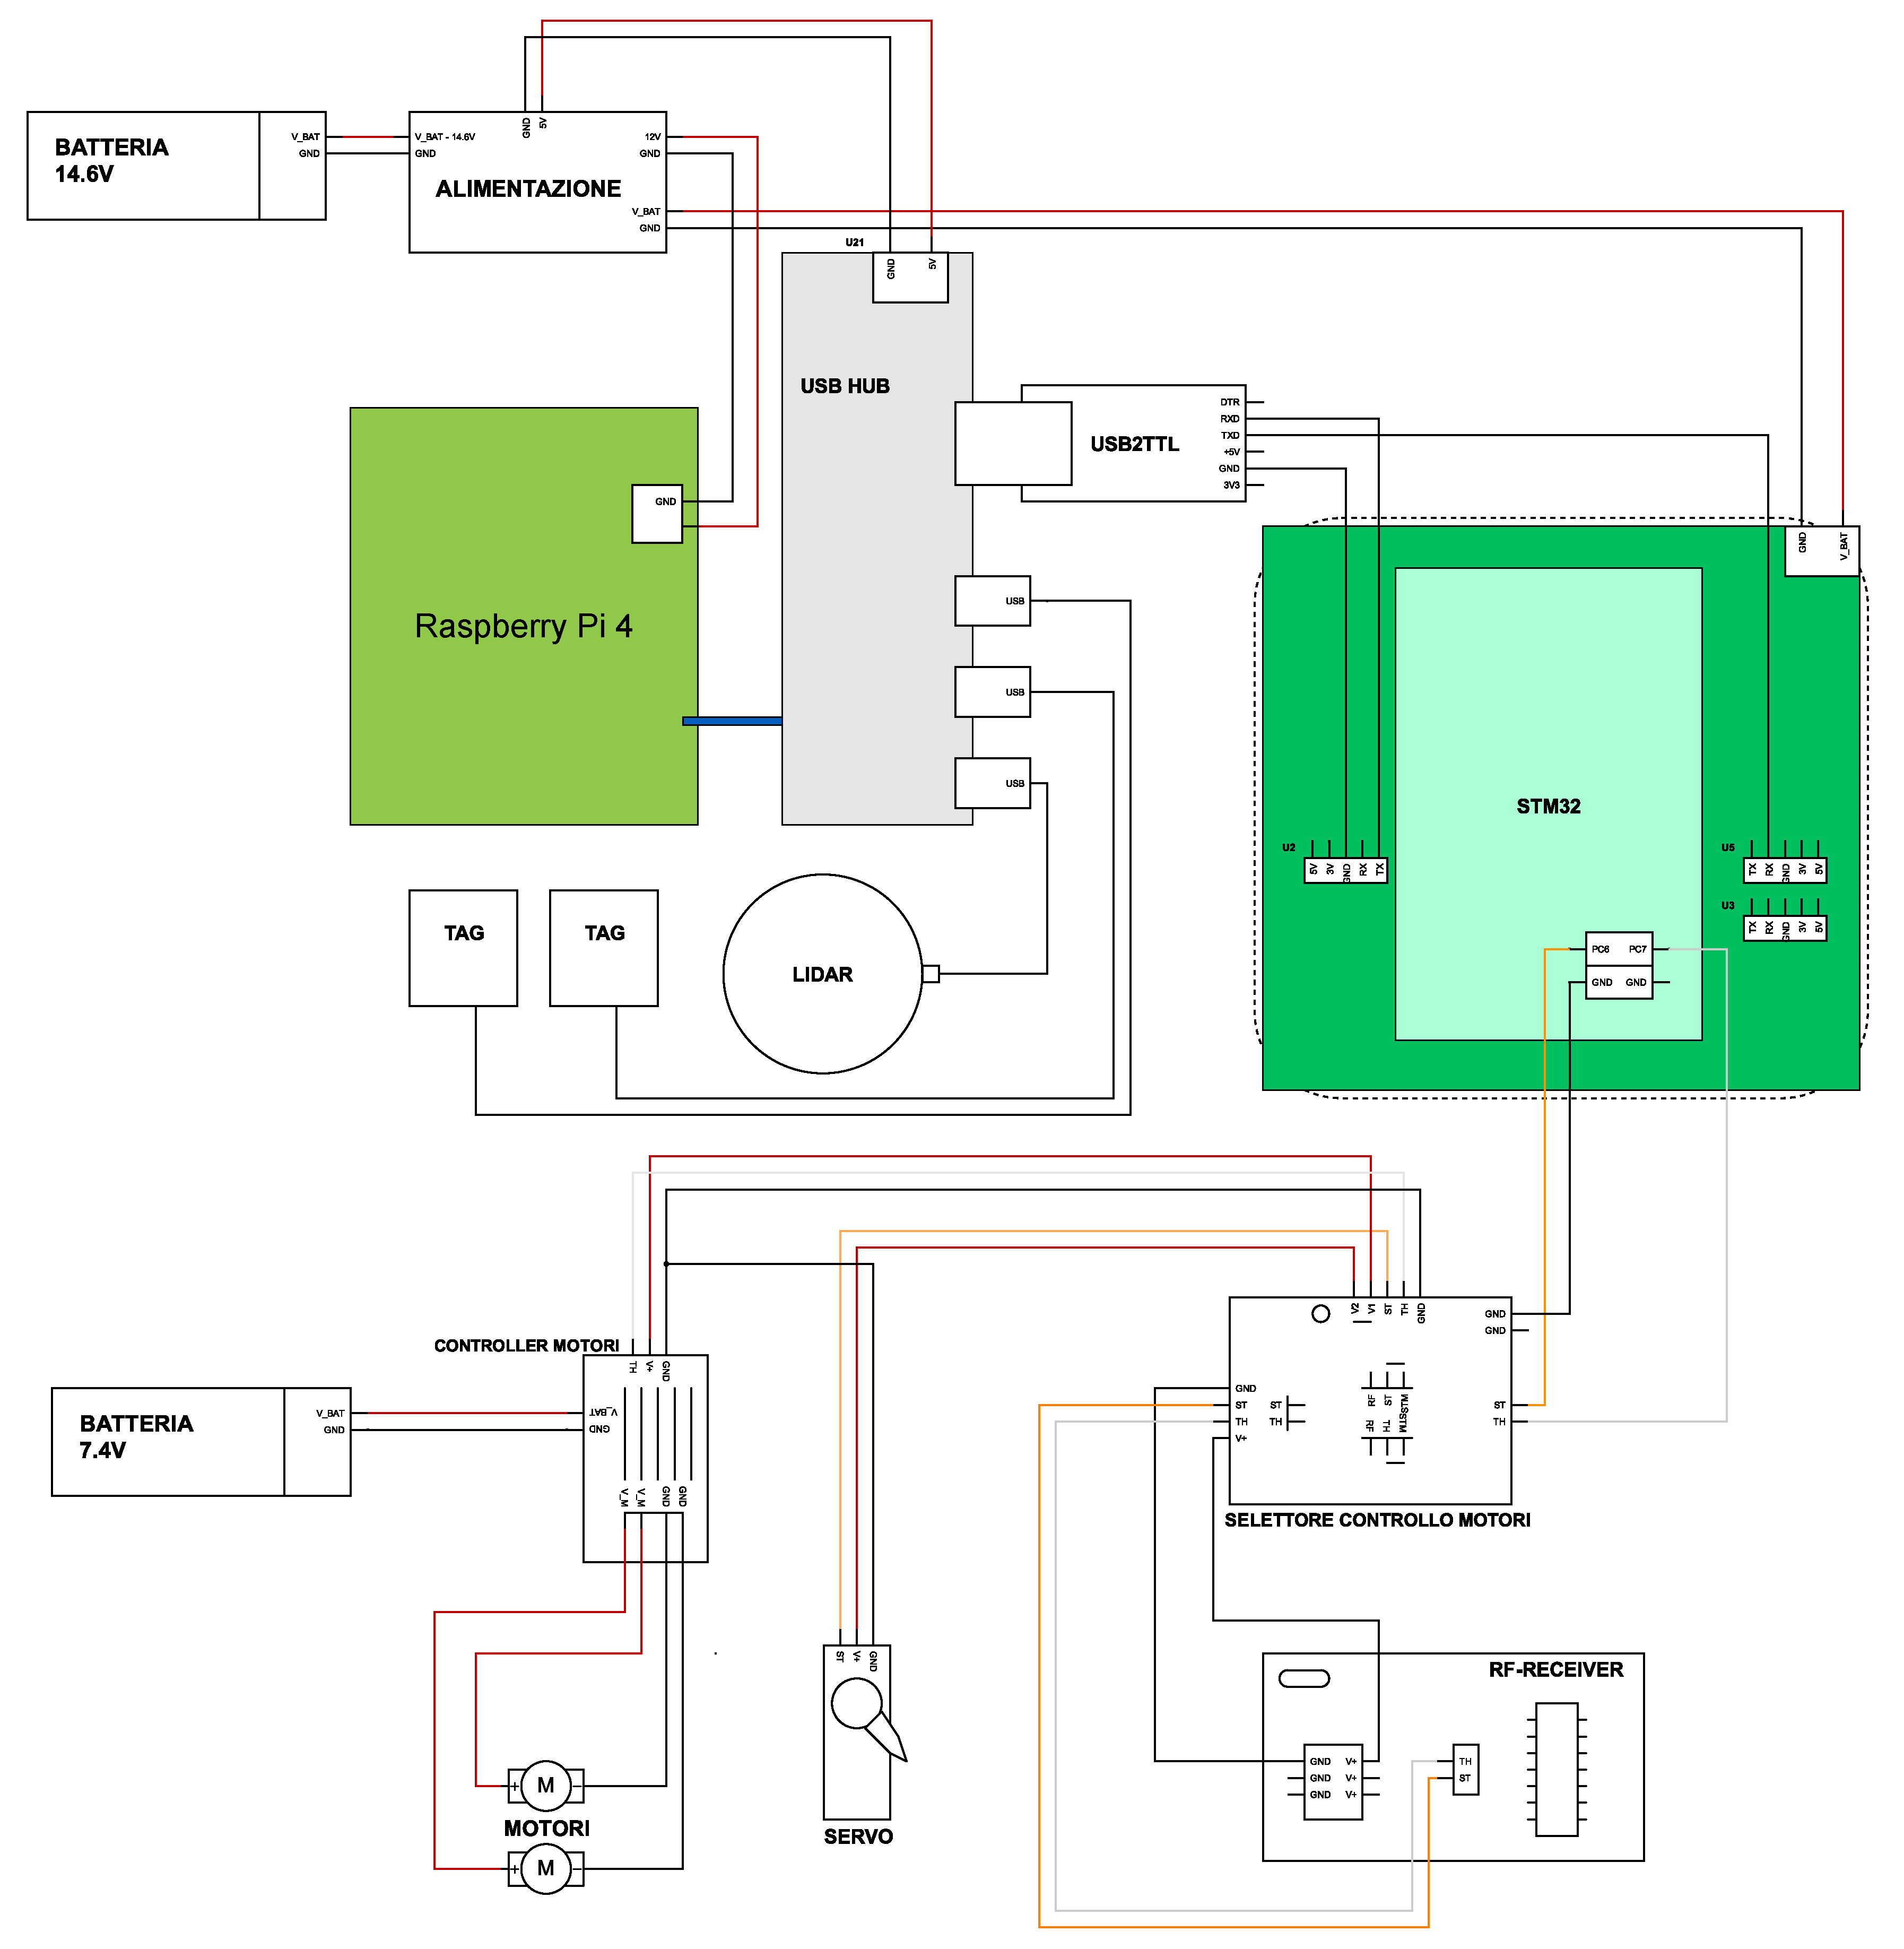
\includegraphics[width=1\textwidth]{schema_completo.pdf}
	\caption{Schema connessioni completo.}
	\label{fig:schema_completo}
\end{figure}

\begin{figure}[] 
	\centering
	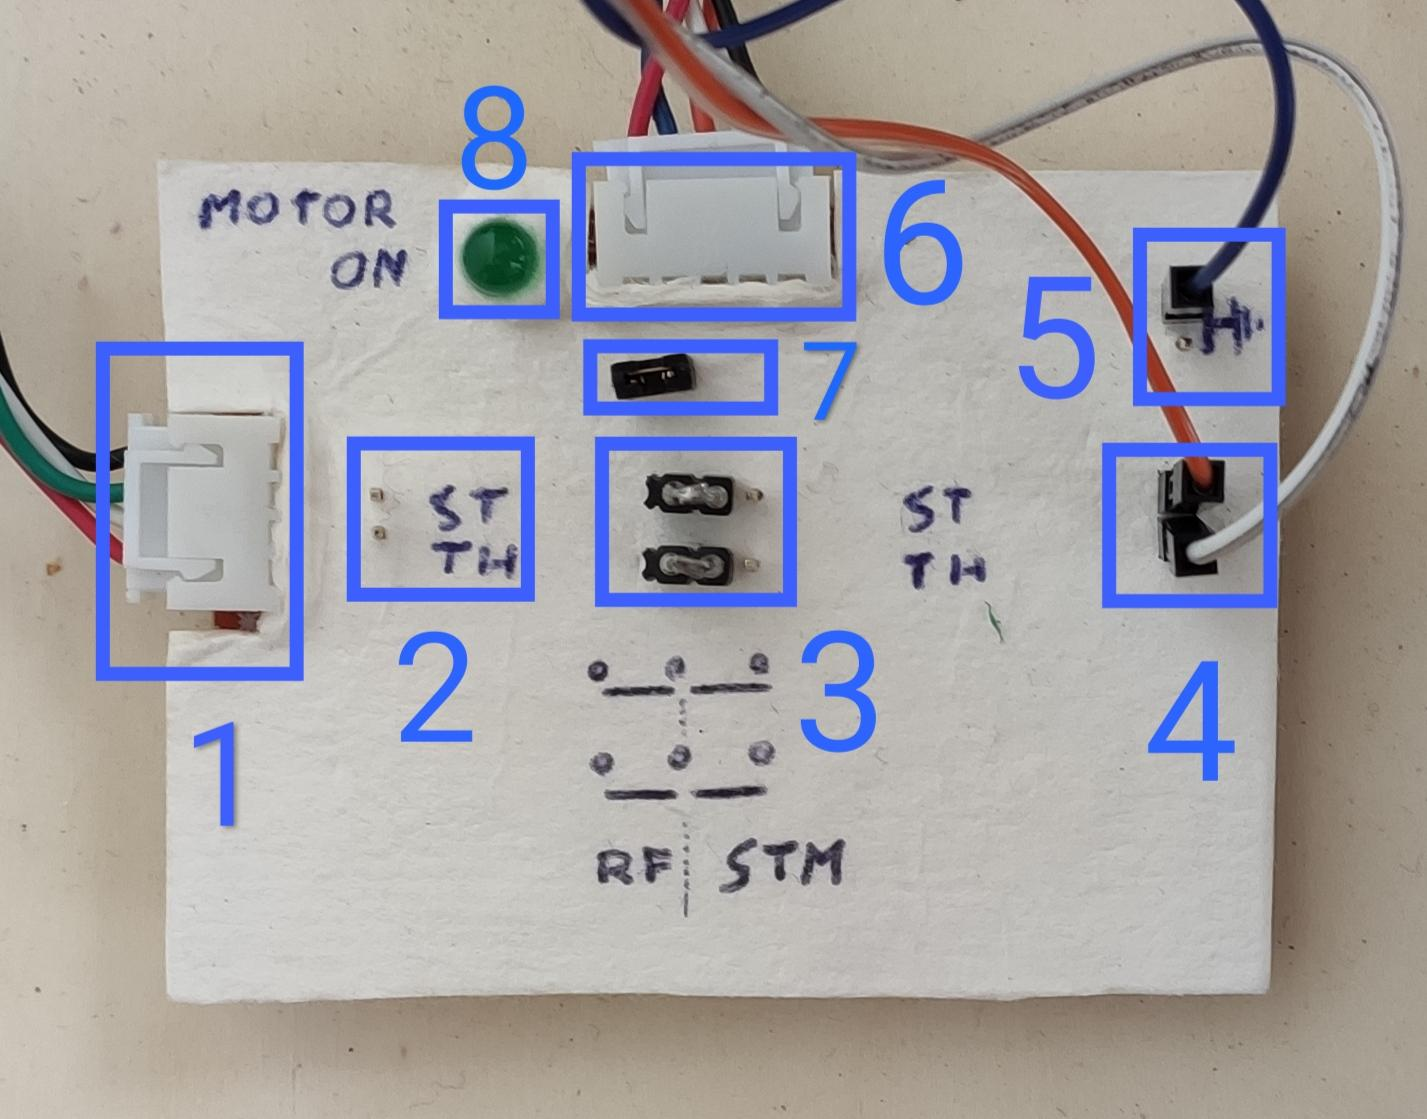
\includegraphics[width=0.45\textwidth]{pcb_controlli.png}
	\caption{PCB controlli}
	\label{fig:pcb_controlli}
\end{figure}


\begin{figure}
	\centering    
	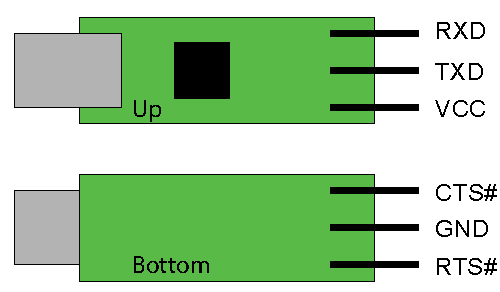
\includegraphics[height=0.2\textheight]{seriale_pinout.pdf}
	\caption{Pinout del convertitore USB-seriale.}
	\label{fig: pinout usbserial}
\end{figure}


Il robot è dotato di due batterie:
\begin{itemize}
	\item LiPo \SI{14.8}{\volt} \SI{4200}{\milli \ampere \hour}, dedicata ad un’alimentazione generica, che viene sfruttata da tutti i componenti tranne i motori; 
	da questa partono 3 linee di alimentazione: 
	\begin{itemize}
		\item a \SI{14.8}{\volt} per la STM
		\item a \SI{5}{\volt} per la Raspberry con connettore usb-c
		\item a \SI{5}{\volt} per fornire alimentazione ausiliaria all’HUB-USB
	\end{itemize}
	\item LiPo \SI{7.4}{\volt} \SI{6000}{\milli \ampere \hour} o NiMH \SI{7.2}{\volt} \SI{3000}{\milli \ampere \hour}, dedicate ai motori
\end{itemize}

I vari convertitori di tensione sono tutti installati su una PCB, posizionata all’interno di un box metallico.

Altro componente fondamentale è il convertitore usb-seriale ``TTL-232R-PCB'' prodotto da 
``Future Technology Devices International Ltd''. 
Questo consente di avere una linea di comunicazione seriale con la STM, attraverso la quale trasmettere informazioni necessarie all'algoritmo di navigazione.
Per conoscere quali informazioni vengono trasmesse, rifarsi alla sez.~\ref{sez:L'esperimento}, mentre per sapere la funzione dei vari pin, si consiglia di 
consultare il datasheet o, più comodamente, di rifarsi alla fig.~\ref{fig: pinout usbserial}. 
Per migliorare la semplicità di utilizzo ed evitare di incorrere in errori legati alle comunicazioni seriali, è stato associato al dispositivo ``TTL-232R-PCB'' 
il symlink \texttt{ttyUSBserial}, in modo tale che l’ordine di inizializzazione delle porte usb della raspberry non influenzi in alcun modo il nome del collegamento 
(per esempio: \texttt{ttyUSB0} oppure  \texttt{ttyUSB1})
Per conoscere i passaggi necessari alla realizzazione di tale symlink, si riporta la procedura dentro il file \texttt{/Info/renaming\_ttyUSB.txt}, 
fornito insieme al codice.


L'algoritmo implementato all'interno dell'STM non è l'unico mezzo attraverso il quale far muovere il veicolo: grazie alla presenza di una piccola PCB, 
sulla quale è presente il circuito adibito allo switch di sistema di controllo e al check dello stato dei motori, si ha la possibilità di utilizzare, 
alternativamente alla STM, un radiocomando per il controllo di sterzo e acceleratore.
Questa PCB, visibile in fig.~\ref{fig:pcb_controlli}, è dotata infatti di un led di stato verde che notifica quando l’alimentazione dei motori è attiva; 
sono inoltre presenti due jumper che permettono di scegliere tra STM e radiocomando come sorgente del controllo per sterzo e acceleratore. 
Sono sempre disponibili all’utente i contatti per potersi connettere e leggere quanto prodotto dal radiocomando.

\begin{enumerate}
    \item Connettore per il ricevitore del radiocomando;
    \item Pin per prelievo segnali PWM (steering/throttle) provenienti dal radiocomando;
    \item Jumper di selezione per la fonte di controllo: (jumper a sinistra) controllo da radiocomando e (jumper a destra) controllo da STM;
	\item Pin per connessione dei canali PWM provenienti da STM (steering/throttle);
    \item Pin per connessione GND comune;
    \item Connettore per i motori;
    \item Jumper di abilitazione alimentazione motori;
    \item LED di stato, indica quando l'alimentazione dei motori è attiva.
\end{enumerate}

Per ulteriori dettagli e approfondimenti sulle scelte che stanno dietro alle connessioni fatte, riferirsi a~\cite{ptvlocalizzazione}.
Lo schema completo è mostrato in fig.~\ref{fig:schema_completo}.

%--------------------------------------------------------
\subsection{Primo collegamento a Raspberry}
\label{sez: primo collegamento a raspberry}

Per iniziare a lavorare sulla raspberry in ssh, modalità richiesta per gli esperimenti, è necessario impostare le connessioni WiFi a cui la raspberry si
connette automaticamente all'avvio. Per comodità di utilizzo, suggeriamo di collegare la raspberry ad un monitor tramite un cavo microHDMI-HDMI e una 
tastiera/mouse usb.

Tutto il necessario da sapere riguardo i passaggi per il primo collegamento a raspberry si trovano nel file: \texttt{Info/README\_wifi\_settings.txt}, dei quali 
riportiamo qui un breve riassunto.
Come prima cosa è va impostato il WiFi: il file con le varie impostazioni WiFi, chiamato \texttt{interfaces}, si trova in \texttt{/etc/network/}. Per editarlo:
\begin{lstlisting}[style=bash]
	sudo nano /etc/network/interfaces
\end{lstlisting}
Questo file si occupa di leggere le configurazioni salvate nei file \texttt{.conf} di cui sono indicati i path al suo interno. 

Per aggiungere una nuova configurazione, inserire una riga per file \texttt{.conf} e commentare le altre (con \#).
Ad esempio, se volessimo aggiungere una configurazione di rete con nome ``NOME\_RETE'', \`e consigliato inserire la seguente riga all'interno del file 
(attenzione: l'ordine conta! Vengono tentate prima le connessioni alle reti riportate più in alto nel file):
\begin{lstlisting}[style=xml]
	wpa-conf /etc/wpa_supplicant/wpa_supplicant_NOME_RETE.conf
\end{lstlisting}
Il file \verb|wpa_supplicant_NOME_RETE.conf| deve contenere:
\begin{lstlisting}[style=xml]
	ctrl_interface=DIR=/var/run/wpa_supplicant GROUP=netdev
	update_config=1
	country=IT

	network={
		ssid="NOME_RETE"
		psk="password"
	}
\end{lstlisting}
e deve essere posizionato nel path specificato. 
Nel caso si usi quello di default, ovvero (\texttt{/etc/wpa\_supplicant/}), si riporta un comando utile per creare un nuovo file:
\begin{lstlisting}[style=bash]
	sudo nano /etc/wpa_supplicant/wpa_supplicant_NOME_RETE.conf
\end{lstlisting}

Al prossimo riavvio la raspberry si connetterà automaticamente alla prima rete configurata (in ordine di righe) che sia disponibile. 
Dato che è già in atto la connessione tramite lo schermo, che permette di visualizzare il contenuto di raspberry, suggeriamo come prima cosa di procedere 
con un backup della scheda originale: esiste un apposito tool all'interno di raspbian che consentirà di farlo agilmente. \`E buona norma creare il backup a 
monte dell'apporto di qualsiasi modifica o aggiunta, in quanto ciò consentirà di avere, in caso di necessità, un punto di ripristino funzionante. 

\subsection{Ros master/slave}
\label{sez: Ros master/slave}
Al fine di non sovraccaricare la raspberry e di avere un'interazione fluida con rviz e altri tool grafici di ros, è fortemente consigliato l'utilizzo di ros su 
altri computer in parallelo, delegando loro l'esecuzione dei task più costosi a livello computazionale (come appunto quelli grafici). 
Sono riportati di seguito i passaggi utilizzati da noi per impostare l'intero sistema, al fine di facilitare i nuovi utenti; per saperne di più consultare la 
\href{https://wiki.ros.org/ROS/Tutorials/MultipleMachines}{guida ufficiale}. 

Dopo svariate prove, siamo giunti alla conclusione che, per arrivare ad avere una interfaccia per utente sufficientemente fluida ed efficace, quello che dovevamo 
fare era avere il RosMaster su raspberry e utilizzare invece il pc per i tool grafici, esempio rviz o rqt. 
Per farlo, dobbiamo ottenere l'ip dei nostri dispositivi: è possibile farlo attraverso vari comandi (come \texttt{ifconfig} o \texttt{ip address}) e generalmente 
risulterà essere qulcosa del tipo: \verb|192.168.43.247|. 
Ipotizziamo quindi che l'ip della raspberry sia \texttt{IPrasp} e quello del pc \texttt{IPpc}. 
Adesso occorre modificare il file \texttt{.bashrc} sia su raspberry che su pc. Iniziamo da pc:
\begin{lstlisting}[style=bashpc]
	nano ~/.bashrc 
\end{lstlisting}
e inseriamo a fine file:
\begin{lstlisting}[style=xml]
	# ROS MASTER SU RASPBERRY, LATO PC
	export ROS_MASTER_URI=http://IPrasp:11311/
	export ROS_HOSTNAME=IPpc
	export ROS_IP=IPpc
\end{lstlisting}

Ripetiamo l'operazione su raspberry:
\begin{lstlisting}[style=bash]
	nano ~/.bashrc 
\end{lstlisting}
e quindi:
\begin{lstlisting}[style=xml]
	% # ROS MASTER SU RASPBERRY, LATO RASPBERRY
	% export ROS_MASTER_URI=http://localhost:11311/
	% export ROS_HOSTNAME=IPrasp
	% export ROS_IP=IPrasp
\end{lstlisting}

A questo punto, è sufficiente riavviare le shell dei terminali che si vogliono utilizzare: sarà possibile in essi lanciare i nodi, installati su pc, 
direttamente dal pc, ma sfruttando il master su raspberry.

%%%%%%%%%%%%%%%%%%%%%%%%%%%%%%%%%%%%%%%%%%%%%%%%%%%%%%%%%%%%%%%%%%%%%%%%%%%%%%%%%%%%%%%%%%%%%%%%%%%%%%
\section{RPlidar}
\begin{figure}[] 
	\centering    
	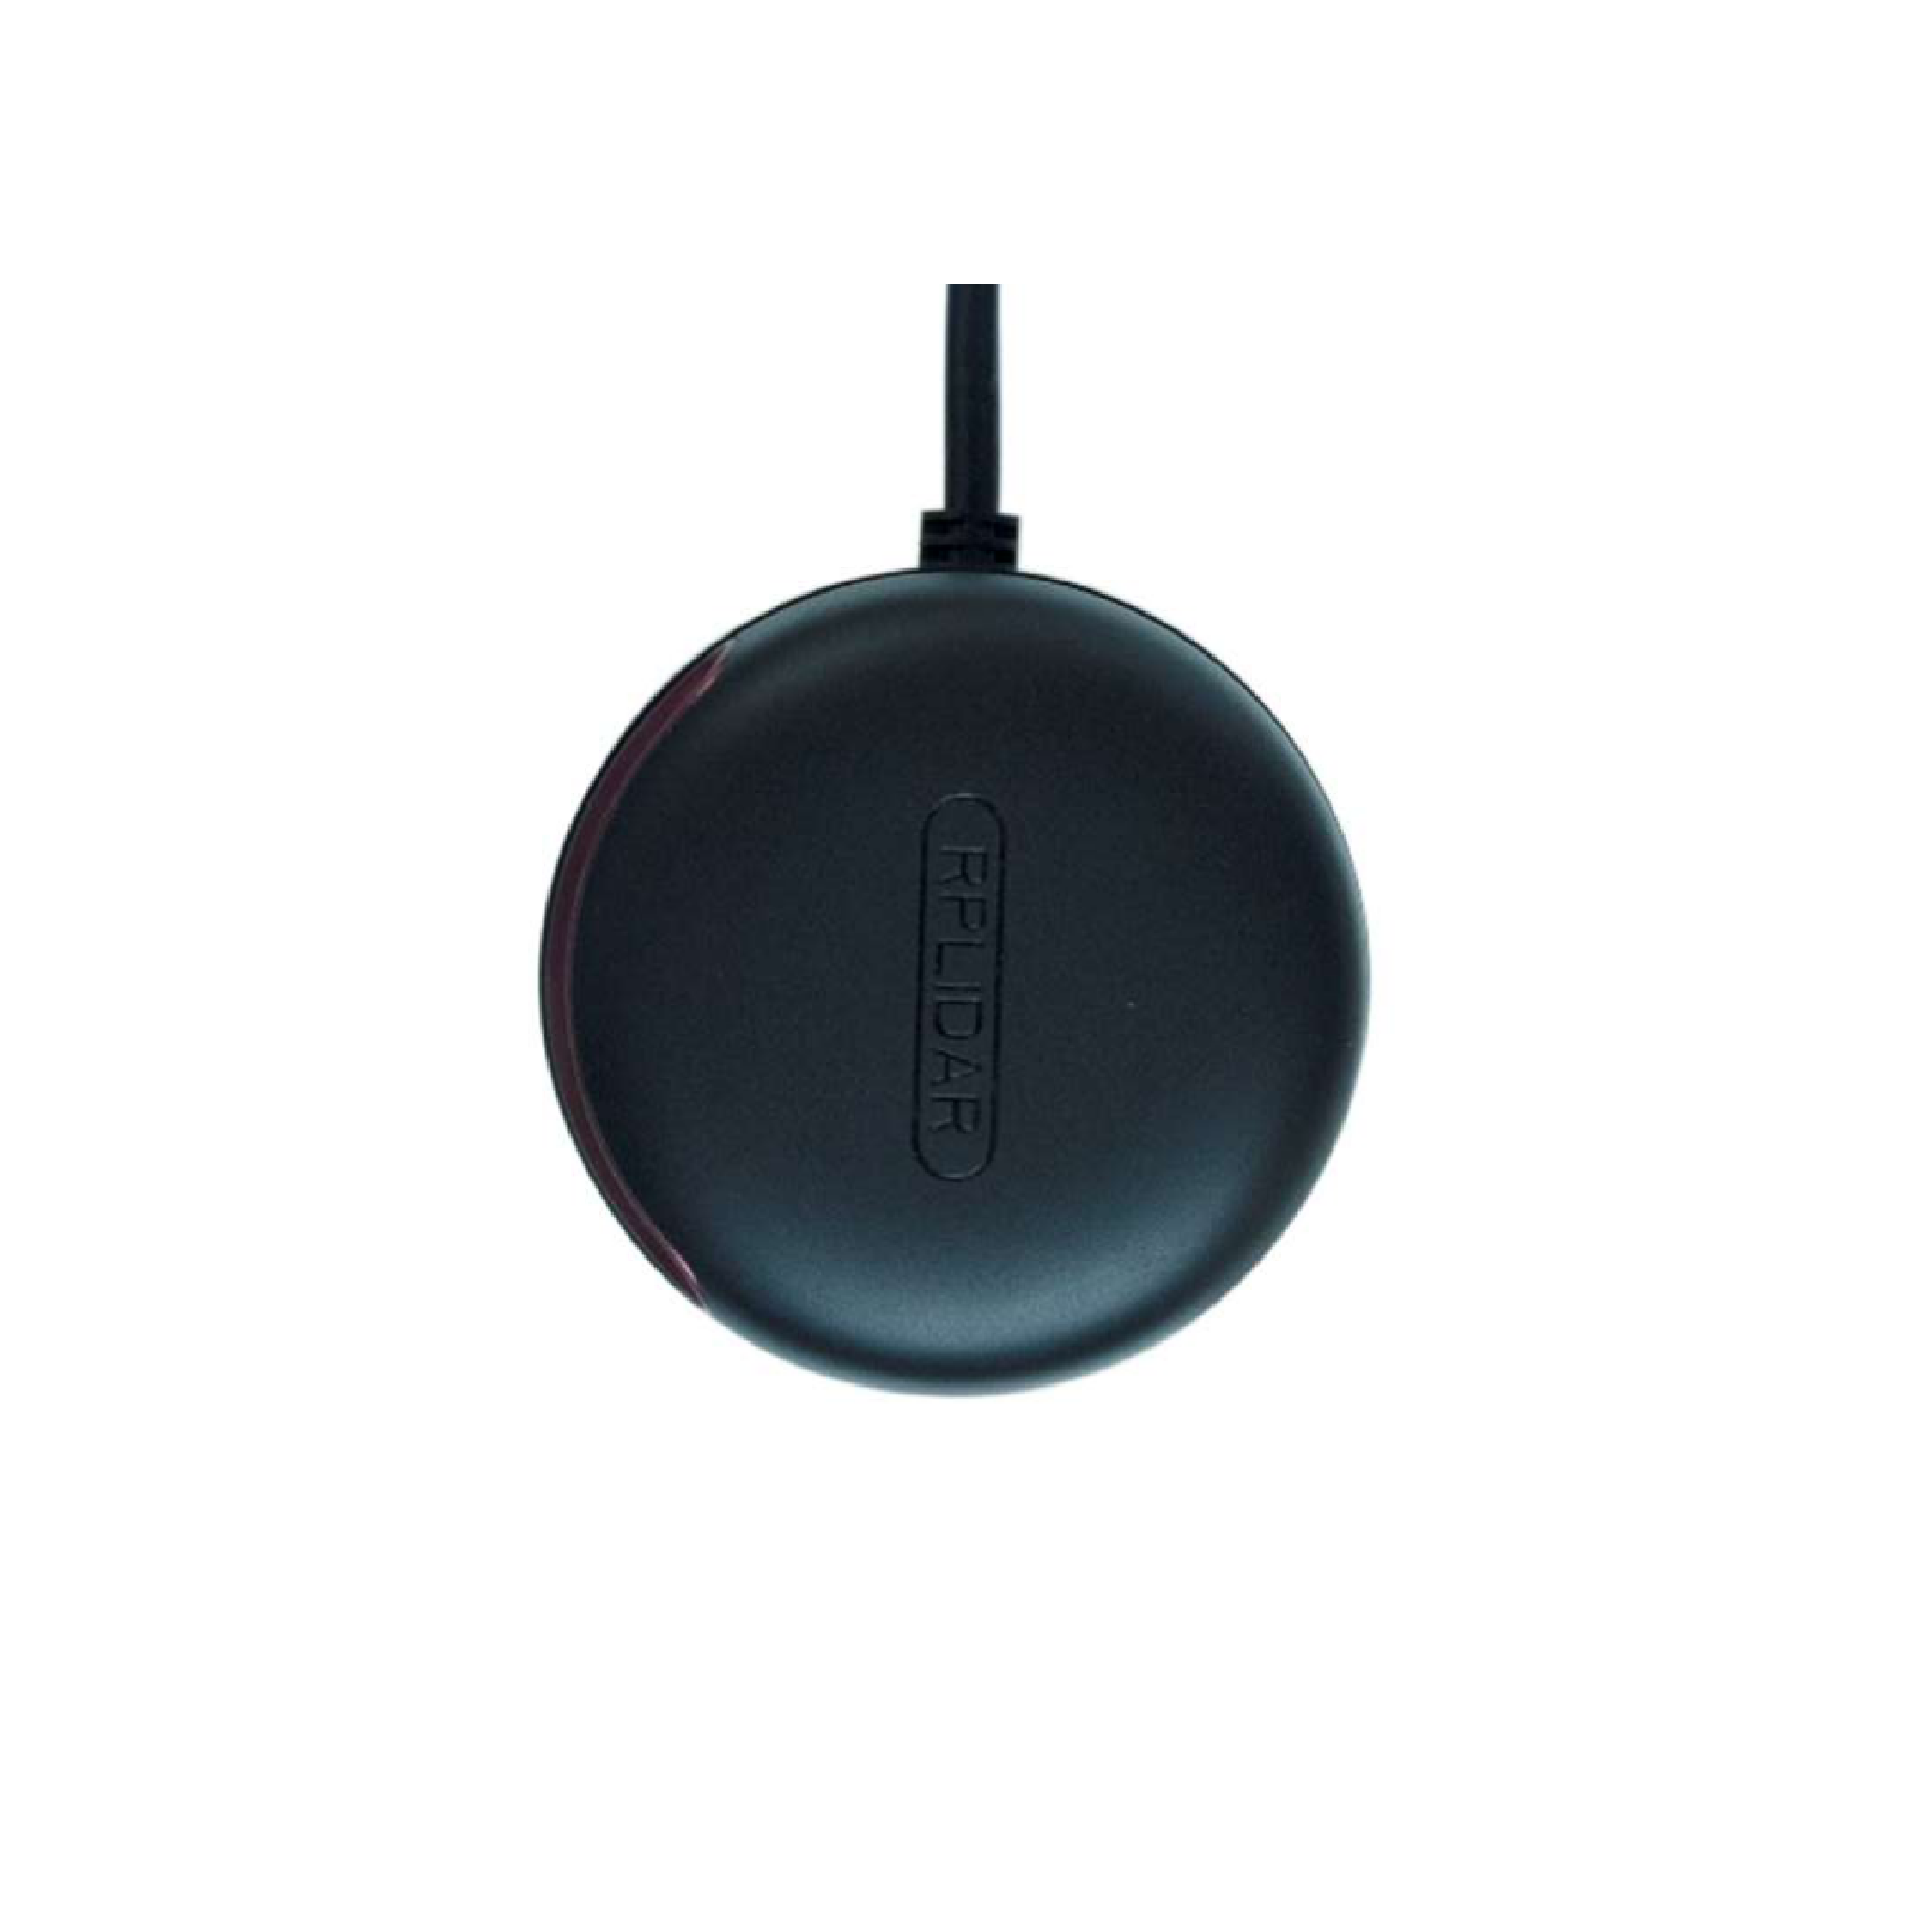
\includegraphics[height=.2\textheight]{rplidar_axis.pdf}
	\caption{Riferimenti}
	\label{fig: rplidar axis}
\end{figure}

Il lidar utilizzato su Charlie è un RPlidar A3 prodotto da Slamtec, di cui documentazione e caratteristiche sono disponibili sulla
\href{https://www.slamtec.com/en/Lidar/A3}{pagina} del produttore.
Per quanto riguarda il codice, abbiamo scelto di utilizzare il \href{https://wiki.ros.org/rplidar}{pacchetto} ros sviluppato proprio da Slamtec. 
Alcune accortezze hardware sono state:

\begin{itemize}
	\item utilizzare un cavo micro usb di buona qualità. Infatti, questo cavo è responsabile sia dell'alimentazione del motore brushless sia della seriale di 
	comunicazione. Ci siamo accorti che, se il voltaggio in ingresso al lidar cala sotto i \SI{4.7}{\volt}, la comunicazione seriale si interrompe e non è più possibile 
	sfruttare i nodi ros di RPlidar.

	\item orientare correttamente il sistema di riferimento del lidar, in quanto le rappresentazioni nel datasheet sono invertite di $\pi$. 
	L'asse x ($\vartheta = 0$), infatti, coincide con l'uscita del cavo dalla struttura principale, come si può vedere in fig.~\ref{fig: rplidar axis}.

	\item cercare di far vibrare il meno possibile la struttura di sostegno e rialzo del lidar.

\end{itemize}

Per evitare, di nuovo, che l'ordine di inizializzazione delle porte usb della raspberry possa influenzare il nome del collegamento (per esempio: 
\texttt{ttyUSB0} oppure \texttt{ttyUSB1}) abbiamo realizzato anche per questo dispositivo il symlink \texttt{ttyUSBlidar}:ciò fa sì che la porta seriale 
del lidar sia sempre chiamata \texttt{ttyUSBlidar}. 
Per realizzare tale symlink, consultare la procedura riportata nel file \texttt{/Info/renaming\_ttyUSB.txt}.

In ambiente ros viene eseguito il lidar andando a lanciare il nodo \texttt{rplidarNode}, il quale pubblica sul topic \texttt{/scan}. 
\`E stato sviluppato il file di lancio \texttt{rplidar\_a3.launch} con i parametri opportuni per il nostro sistema.  
Per quanto riguarda l'utilizzo del lidar, non è stato necessario alcun sviluppo software in quanto il pacchetto ros risulta già completo.


%%%%%%%%%%%%%%%%%%%%%%%%%%%%%%%%%%%%%%%%%%%%%%%%%%%%%%%%%%%%%%%%%%%%%%%%%%%%%%%%%%%%%%%%%%%%%%%%%%%%%%
\newpage
\section{Sistema Pozyx}
\label{sez:Sistema Pozyx}

\begin{figure}[h]
	\centering
	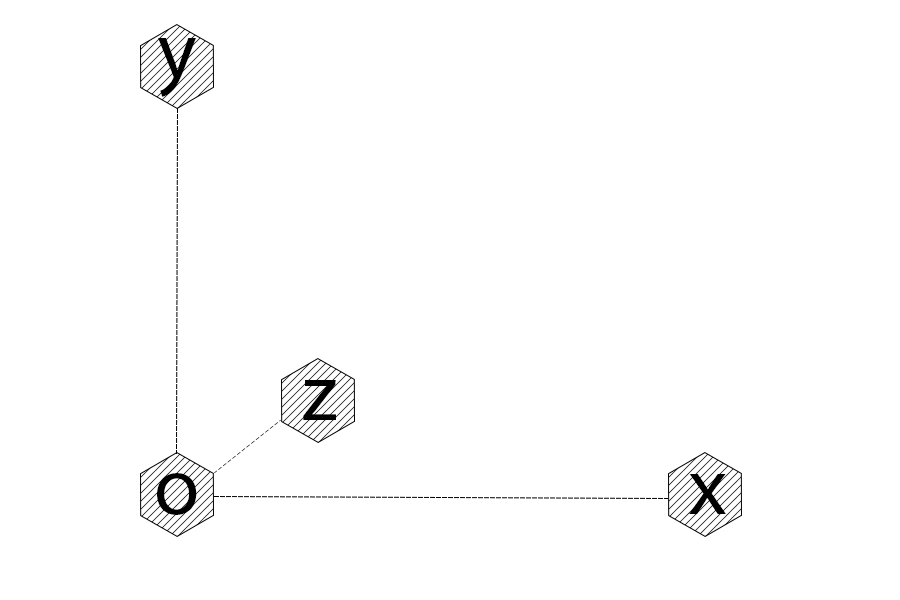
\includegraphics[height=0.2\textheight]{uwb_axis.png}
	\caption{Disposizione ancore}
	\label{fig: disposizione ancore}
\end{figure}


Il Pozyx è un sistema di localizzazione alternativo al GPS, basato sulla tecnologia ultra-wideband
(UWB). In breve, si tratta di una tecnica per la trasmissione e la ricezione di segnali sviluppata in modo tale che vengano sfruttati impulsi di energia 
a radiofrequenza aventi durata temporale molto ridotta (nanosecondi), con conseguente banda spettrale ampia.
Nel sistema Pozyx si possono distinguere due entità, ciascuna con le proprie peculiarità: le ancore e le tag.
La configurazione base prevede l'utilizzo 4 ancore, che fungono da dispositivi fissi, e una tag, che rappresenta il dispositivo mobile.
Grazie all'utilizzo di un algoritmo di triangolazione, la tag si può localizzare rispetto alle ancore. Teoricamente, la localizzazione tramite tecnologia 
ultra-wideband permette di ottenere un posizionamento con una accuratezza al centimetro anche
in ambienti indoor e in presenza di ostacoli di natura non metallica, condizioni sfavorevoli per il sistema (che presenta 
migliori performance in ambienti aperti ed ampi, privi di oggetti metallici e ostacoli sui quali possano verificarsi fenomeni di scatterning 
del segnale inviato). 
Sia all'interno delle tag che delle ancore è presente un microcontrollore, nel quale vengono eseguiti la maggior parte dei task richiesti,
come gli algoritmi di triangolazione e autocalibrazione. A lui è demandata anche la gestione dell’interfaccia con dispositivi esterni
(come Arduino).
Solo nel caso delle tag, che per questo sono utilizzate come dispositivi mobili, sono presenti i seguenti sensori: un magnetometro, un giroscopio, un
accelerometro e un sensore di pressione (altimetro). I dati dei sensori vengono utilizzati dal microcontrollore
per la triangolazione e sono disponibili all’utente.
Per quanto riguarda l'utilizzo di tale sistema di posizionamento, è necessario prima di tutto predisporre l'ambiente di lavoro.
La prima cosa da fare è posizionare le ancore in modo tale che delimitino uno spazio entro il quale il sistema di localizzazione
funzioni correttamente. Il miglior modo di disporle è quello di metterle in alto e sulla line-of-sight dell’utente: questo tipo di scelta
aumenta la possibilità di ricevere un buon segnale, in quanto permette di limitare la presenza di possibili ostacoli. 
Per un buon funzionamento e per ridurre il più possibile l'errore di posizionamento, è consigliato inoltre distribuire le ancore affinché tutte le 
direzioni siano coperte.
Nel caso, infatti, in cui gli ancoraggi si trovino su una linea retta, l'errore di posizionamento risultante sarebbe molto grande e potrebbero
verificarsi ambiguità di posizione legate alla simmetria della configurazione.
Per un buon funzionamento del sistema, è infine importante disporre le ancore verticalmente e con l’antenna UWB rivolta verso l’alto.

Una volta predisposto l'ambiente di lavoro, si passa alla parte di comunicazione tra i vari agenti in gioco. Per tutte le operazioni che vengono richieste 
tra le ancore e le tag, è necessario specificare tra quali dispositivi lavorare. 
Con l'identificativo assegnato al campo \verb|remote_id|, si dichiara la tag o l'ancora sulla quale vogliamo usare le funzioni di registro. Nel caso (di default) 
in cui questo sia settato al valore \verb|None|, verrà usata la tag locale, ovvero quella connessa al pc (su cui viene utilizzata la seriale).
Presa ad esempio la funzione doRanging(destination, \verb|device_range|, \verb|remote_id=None|), essa effettua una misurazione della distanza tra i dispositivi
i cui identificativi sono \verb|remote_id| e destination. Lasciando il valore di default per \verb|remote_id|, cioè \verb|None|, la distanza viene automaticamente
valutata tra il dispositivo connesso alla seriale del PC e il dispositivo il cui identificativo è destination. 
Se si desidera, invece, che il ranging venga effettuato tra due diversi dispositivi della rete, basterà inserire l’opportuno valore di \verb|remote_id|.

Nel nostro caso, questo aspetto risulta essere fondamentale nel momento in cui vengono prelevate le posizioni relative delle ancore nella configurazione corrente. 

Con \verb|remote_id=None|, chiediamo di fatto alla tag connessa in seriale ad Arduino di fornirci le informazioni delle ancore, ovvero leggiamo sul suo chip i valori 
relativi all'ancora richiesta (posizione, id...).
Per questo motivo, ad ogni nuovo avvio del sistema è necessario salvare all'interno delle tag i valori di posizione più recenti delle ancore, ovvero gli ultimi 
salvati all'interno delle ancore stesse al termine del processo di autocalibrazione.
Affinché il sistema funzioni, è infatti necessario che ogni ancora abbia coscienza della propria posizione rispetto alle altre ancore: la procedura di 
autocalibrazione è quella utilizzata a tale scopo.
Per informazioni inerenti alla procedura adottata, vedere app.~\ref{sez:Autocalibrazione}. Per come è stati scritto l'algoritmo in questione, l'ancora 0 è quella 
la cui posizione fornisce l'origine del frame UWB che verrà costruito. 
L'ancora 1 indica invece la direzione dell'asse y, ovvero le sue coordinate finali saranno \verb|(0, y1, 0)|, così come l'ancora 2 quella dell'asse x. La quarta 
ancora, posizionata a una altezza diversa dalle altre 3 (che devono invece essece complanari), evidenzia infine la direzione dell'asse z.

Infine, è importante verificare che siano assenti eventuali interferenze elettromagnetiche tra i dispositivi, le quali, specialmente se interposte tra le ancore, 
possono rendere difficile la comunicazione tra i dispositivi della rete.

Per quanto riguarda la componente software, sono stati utilizzati nodi custom basati sul modulo Python di PyPozyx, rispetto ai quali abbiamo apportato modifiche 
per adattarli al nostro sistema. Per maggiori dettagli, vedere nella cartella:
\begin{verbatim}
	...\Workspace\src\charlie_pozyx\src\scripts\my_pozyx 
\end{verbatim}
dove all'interno di ciascun nodo è presente una breve descrizione del suo funzionamento e della sua utilità.

\vspace{0.5 cm}
su uno di questi nodi, ovvero il \verb|pos_pub_2_tag.py|, descriviamo un errore che abbiamo riscontrato e che, plausibilmente, è stato una causa
di errori nelle esecuzioni precedenti. Prima di tutto, questo nodo si occupa di pubblicare la posa delle due tag (posizione + quaternione) e sfrutta al suo interno 
la funzione, sempre custom, \verb|doPos_pubtf|, all'interno della quale è fatto girare l'algoritmo \verb|doPositioning|. Questo, a sua volta, ricava la posizione
delle tag pozyx connesse in seriale. Come spiegato in \cite{ctesconistudio}, l'algoritmo \verb|doPositioning| viene eseguito utilizzando la modalità 
\verb|POZYX_RANGE_PROTOCOL_PRECISION| e questa richiede l'utilizzo di molti sample. Per questo motivo, dato che il \verb|doPositioning| deve essere eseguito 
in modo sequenziale prima sulla tag0, poi sulla tag1, poi nuovamente sulla tag0 e così via, si rende necessario l'inserimento di una pausa tra una esecuzione 
e la successiva, per permettere all'algoritmo di terminare prima di essere lanciato nuovamente. In assenza di tali pause temporali, abbiamo infatti notato che 
i risultati venivano corrotti: dopo l'aggiunta di tali intervalli, invece, le esecuzioni successive non si influenzano più a vicenda, come voluto.

\subsection{Autocalibrazione ancore Pozyx}
\label{sez:Autocalibrazione}
L'autocalibrazione si basa sullo script \texttt{python3} ``autocalibration\_ransac.py''. 
Affinché possa funzionare, occorre per prima cosa avere quattro ancore correttamente alimentate ed un dispositivo Pozyx connesso, il quale servirà da comunicazione 
seriale tra la rete Pozyx e l’utente. 
Il dispositivo seriale può, a discrezione dell’utente, essere un’ancora o un tag. 
É possibile, se si desidera, effettuare una calibrazione manuale delle ancore, andando a settare la variabile \verb|autoCal| a \verb|True|. 
In tal caso, si dovrà innanzitutto utilizzare un metro col quale misurare la distanza relativa tra le coppie di ancore della rete. Queste misure andranno poi 
inserite manualmente  nelle opportune variabili \texttt{r01}, \texttt{r02}, \texttt{r03}, \texttt{r12}, \texttt{r13} ed \texttt{r23}, che rappresentano per l'appunto 
le distanze tra le rispettive antenne.
Per quanto riguarda invece la calibrazione automatica, lo script prevede una prima fase nella quale si ha l'acquisizione dei dati necessari, seguita dall'esecuzione 
l’algoritmo ransac. Infine, viene utilizzato l’algoritmo algebrico per determinare le coordinate effettive delle ancore. 
L’algoritmo ransac permette di rimuovere eventuali outliers dalle misurazioni delle distanze relative tra le antenne e fornisce, quindi, una stima della distanza 
tra ciascuna coppia di ancore basata sui dati senza outliers.
Nel corso della procedura di autocalibrazione vengono stampati sul terminale vari dati, tra cui i fondamentali sono:
\begin{itemize}
	\item Le coordinate dei dispositivi all’accensione del sistema, prima che sia effettuata la nuova calibrazione.
	
	\item Il risultato del settaggio dei parametri UWB della rete.
	
	\item Il risultato dell’algoritmo ransac per la distanza tra le ancore senza outliers.
	
	\item Il risultato dell'algoritmo algebrico per determinare le coordinate delle ancore: in caso di fallimento dell'algoritmo, è mostrato a terminale l'errore.
\end{itemize}

Una volta terminata la calibrazione, sia questa stata manuale o automatica, ciascuna ancora avrà
salvato nella propria lista dei dispositivi le proprie coordinate, ossia potremmo dire che conoscerà le proprie coordinate. 
Questi dati sono salvati permanentemente nella memoria flash.
In una successiva fase di positioning è quindi buona norma che il dispositivo che si deve localiz-
zare interroghi le ancore per conoscere la loro posizione e crei quindi, con queste informazioni, una propria lista interna dei
dispositivi della rete.


Per maggiori approfondimenti, fare riferimento al dettagliato lavoro~\cite{ctesconistudio}.

%%%%%%%%%%%%%%%%%%%%%%%%%%%%%%%%%%%%%%%%%%%%%%%%%%%%%%%%%%%%%%%%%%%%%%%%%%%%%%%%%%%%%%%%%%%%%%%%%%%%
\section{Sistema Vicon}
\label{sez:Sistema Vicon}

Il sistema Vicon è un sistema molto accurato di motion capture. 
In questo progetto è stato utilizzato per fornire un \textit{ground-truth} e un confronto all'algoritmo di navigazione, del quale possiamo così valutare la bontà. 
In tal senso, quindi, abbiamo ritenuto opportuno sviluppare i nodi e i topic di dialogo con il sistema Vicon all'esterno del workspace della raspberry: infatti, 
questi si trovano su pc nel pacchetto in \texttt{charlie\_remote}.

Per poter dialogare con il sistema Vicon, è sufficiente includere nel proprio \texttt{catkin\_ws} il pacchetto \texttt{vrpn\_client\_ros}, disponibile sulla 
\href{https://wiki.ros.org/vrpn_client_ros}{wiki.ros} e scaricabile dalla \href{https://github.com/ros-drivers/vrpn_client_ros}{repo GitHub}.
Questo pubblicherà la posa, il twist e l'accelerazione di ogni oggetto selezionato nel software di tracking (maggiori dettagli su quali oggetti selezionare 
nelle sezioni \ref{sez:L'esperimento} e \ref{sez: Guida breve all'esperimento}).

\subsubsection*{Creazione oggetto}
\label{sez:Sistema Vicon_oggetto}
Nonostante siano già presenti gli oggetti necessari per il tracking di Charlie, riportiamo la procedura di creazione di un nuovo oggetto, la quale potrebbe essere
utile in caso di modifiche ai marker o in altre circostanze. 
Sinteticamente è necessario procedere come segue:
\begin{enumerate}
	\item Disporre 4 o più marker sull'oggetto desiderato in modo asimmetrico. Per facilitare i passi successivi, è consigliato disporre alcuni marker sugli assi 
	del sistema di riferimento body.
	
	\item Selezionare i marker nell'applicazione ``Vicon Tracker 3.7.0 x64'' semplicemente clickando e tenendo premuto il tasto sinistro del mouse, poi premere 
	pausa (pulsante collocato a sinistra).
	
	\item spostarsi nel tab Objects, assegnare un nome in basso e premere Create Object. L'applicazione assegna un sistema locale di default.
	
	\item Modificare il sistema locale premendo sugli assi o accedendo nelle proprietà dell'oggetto appena creato. Una volta soddisfatti, premere \texttt{Ctrl+S} 
	per salvare l'oggetto.
	
	\item Premere di nuovo il pulsante di pausa e verificare che il tracciamento stia funzionando.
\end{enumerate}
           
\subsubsection*{Calibrazione}
Per effettuare una calibrazione del sistema, necessaria di tanto in tanto affiché il motion capture non accumuli errori dovuti a cambiamenti delle condizioni 
dell'ambiente o a piccoli spostamenti delle camere, è necessario utilizzare la wand. 
La procedura richiesta si compone dei seguenti passi, riportati sempre in via sintetica. Per prima cosa, è necessario accedere all'applicazione 
``Vicon Tracker 3.7.0 x64'' e collocarsi nella tab ``Calibrate''. 
Premere poi su ``Start'' nella sezione ``CALIBRATE CAMERAS'', avviando così la procedura di autocalibrazione: spostare la wand con pattern circolari 
all'interno della stanza assicurandosi di avere sempre più camere ``a vista''. 
Il software interromperà da solo l'acquisizione dei dati una volta che questi risultino essere sufficienti.

Adesso è necessario definire il sistema di riferimento. Per fare questo, andiamo a posizionare l'incrocio degli assi della wand nel punto in cui vogliamo 
l'origine e gli assi stessi dell'oggetto in modo che siano allineati con gli assi-Vicon desiderati.
Selezioniamo quindi il marker all'incrocio come origine e gli altri marker come asse x e asse y, completando così la calibrazione del sistema. 
Nella stanza del volo del DII, il sistema di riferimento più usato è rappresentato in fig.~\ref{fig: stanza volo Vicon frame}.

\begin{figure}[] 
	\centering    
	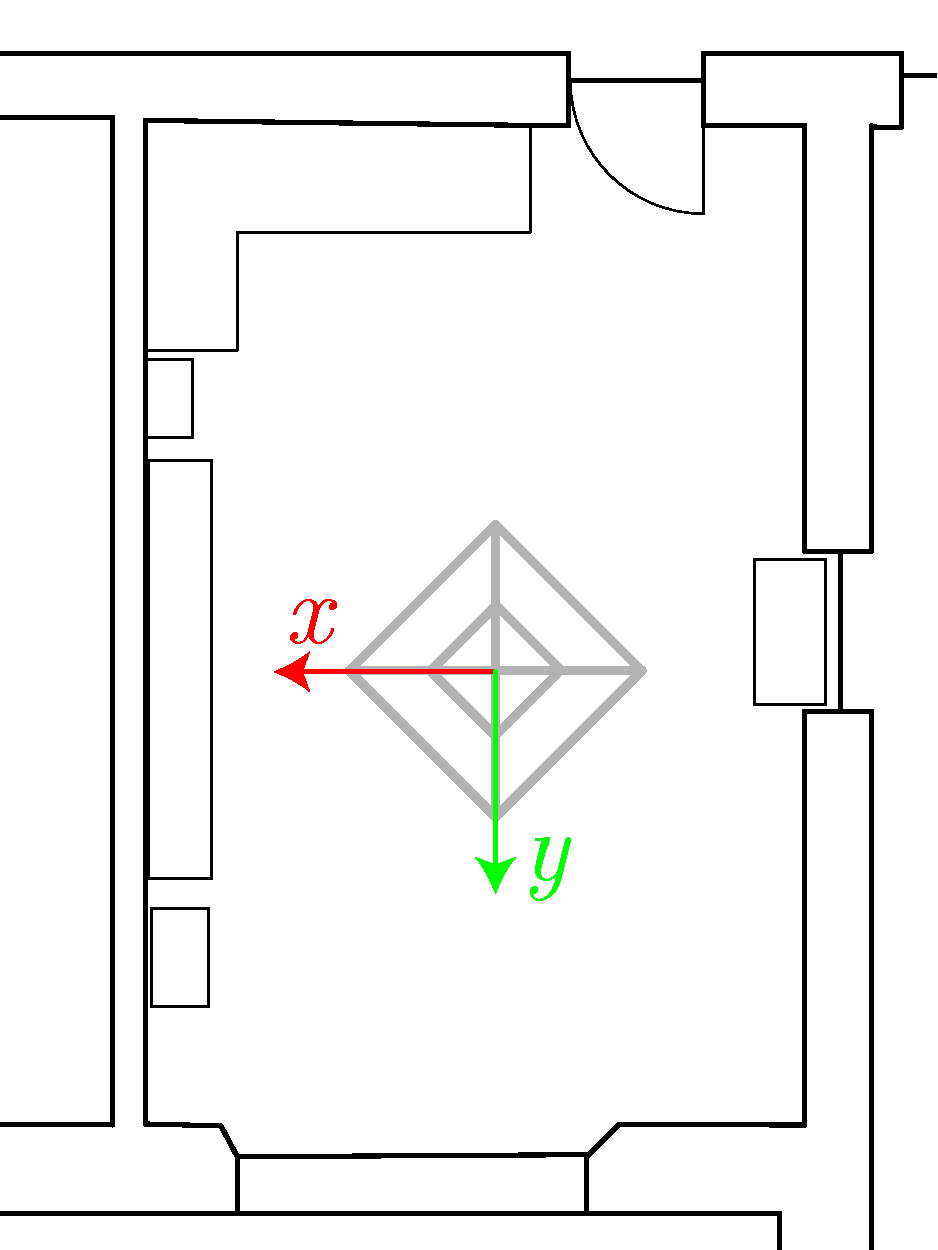
\includegraphics[height=.4\textheight]{stanza_volo.pdf}
	\caption{stanza volo}
	\label{fig: stanza volo Vicon frame}
\end{figure}


%%%%%%%%%%%%%%%%%%%%%%%%%%%%%%%%%%%%%%%%%%%%%%%%%%%%%%%%%%%%%%%%%%%%%%%%%%%%%%%%%%%%%%%%%%%%%%%%%%%%%%
\newpage
\section{Ambiente ROS creato}
\label{sez:Ambiente ROS creato}
In questa sezione delineiamo l'ambiente ros realizzato. 
Vista la naturale confusione che si era accumulata nei passaggi di testimone da gruppo a gruppo, abbiamo deciso di ricostruire l'ambiente ros da capo aggiornandolo da ros kinetic a ros melodic; questa scelta \`e venuta spontanea dall'aver cambiato di processore, da intel Joule con Ubuntu 16.04 a Raspberry Pi 4 con Ubuntu 18.04.
Facendo attenzione ai singoli pacchetti utilizzati e controllando ogni nodo utilizzato siamo stati in grado di individuare codice superflue e alcuni piccoli ma decisivi errori.

\subsection{Pacchetti utilizzati}
Passiamo adesso a descrivere i singoli packages utilizzati.
ulteriori informazioni  sui pacchetti, sulle loro dipendenze e come installarli sono riportate in \verb|Info/Pacchetti.ods| e in \verb|readme_packages.txt|.
\subsubsection*{Ambiente charlie\_ws}
Questo ambiente \verb|catkin| \`e caricato sulla raspberry e ha lo scopo di localizzare il veicolo.
I pacchetti utilizzati sono riportati in tab.~\ref{tab: pacchetti charlie}.

\begin{table}[h]
	\centering
	\begin{tabular}{lcp{0.5\linewidth}}
		\textit{Nome} 	& \textit{Origine} & \textit{Descrizione} \\
		\hline
		charlie\_launch				& Custom	& File di lancio per l'esperimento.\\
		geometry2-melodic-devel		& Ros		& Stack ROS legato a tf2.\\
		hector\_slam				& Ros		& Stack ROS per fare SLAM, utilizzato da noi per creare la mappa.\\
		navigation					& Ros		& Stack di navigazione. Contiene \verb|amcl|.\\
		navigation\_msgs			& Ros		& Stack ROS per definire i messaggi di navigazione.\\
		pcl\_msgs-indigo-devel		& Ros		& Messaggi legati a PCL ROS.\\
		perception\_pcl				& Ros		& Point Cloud Library, collezione di algoritmi per processare Point Clouds in n-Dimensioni e geometria 3D.\\ 
		pozyx\_ros					& Custom	& Pacchetto sviluppato per comunicare con il sistema Pozyx uwb, per eseguire posizionamento e altro.\\
		rplidar\_ros				& Ros		& Pacchetto per comunicare e pubblicare le scansioni del lidar.\\
		scan\_tools					& Ros		& Stack ROS che contiene strumenti per manipolare \verb|sensor_msgs/LaserScan| e \verb|sensor_msgs/PointCloud|.\\
		SerialManager				& Custom	& Pacchetto sviluppato per comunicare alla scheda STM i topic necessari all'esperimento.\\
	\end{tabular}
	\caption{Elenco pacchetti utilizzati}
	\label{tab: pacchetti charlie}
\end{table}
\FloatBarrier
	
\subsubsection*{Ambiente charlie\_remote\_ws}
Da PC, remoto insomma, abbiamo utilizzato gli strumenti grafici non necessari all'esperimento ma utili come ad esempio \verb|rviz|. I pacchetti utilizati sono riportati in tab.~\ref{tab: pacchetti remoto}
\begin{table}[h]
	\centering
	\begin{tabular}{lcp{0.5\linewidth}}
		\textit{Nome} 	& \textit{Origine} & \textit{Descrizione} \\
		\hline
		charlie\_remote			& Custom	& File di lancio per tool grafici dell'esperimento e nodi di trasformazione dal frame Vicon.\\
		vrpn\_client\_ros		& Ros		& Pacchetto ROS che include il necessario per la comunicazione con il sistema Vicon.\\
	\end{tabular}
	\caption{Elenco pacchetti utilizzati da PC}
	\label{tab: pacchetti remoto}
\end{table}
\FloatBarrier

	
\subsection{Nodi e topic utilizzati}

\begin{figure}[h]
	\centering
	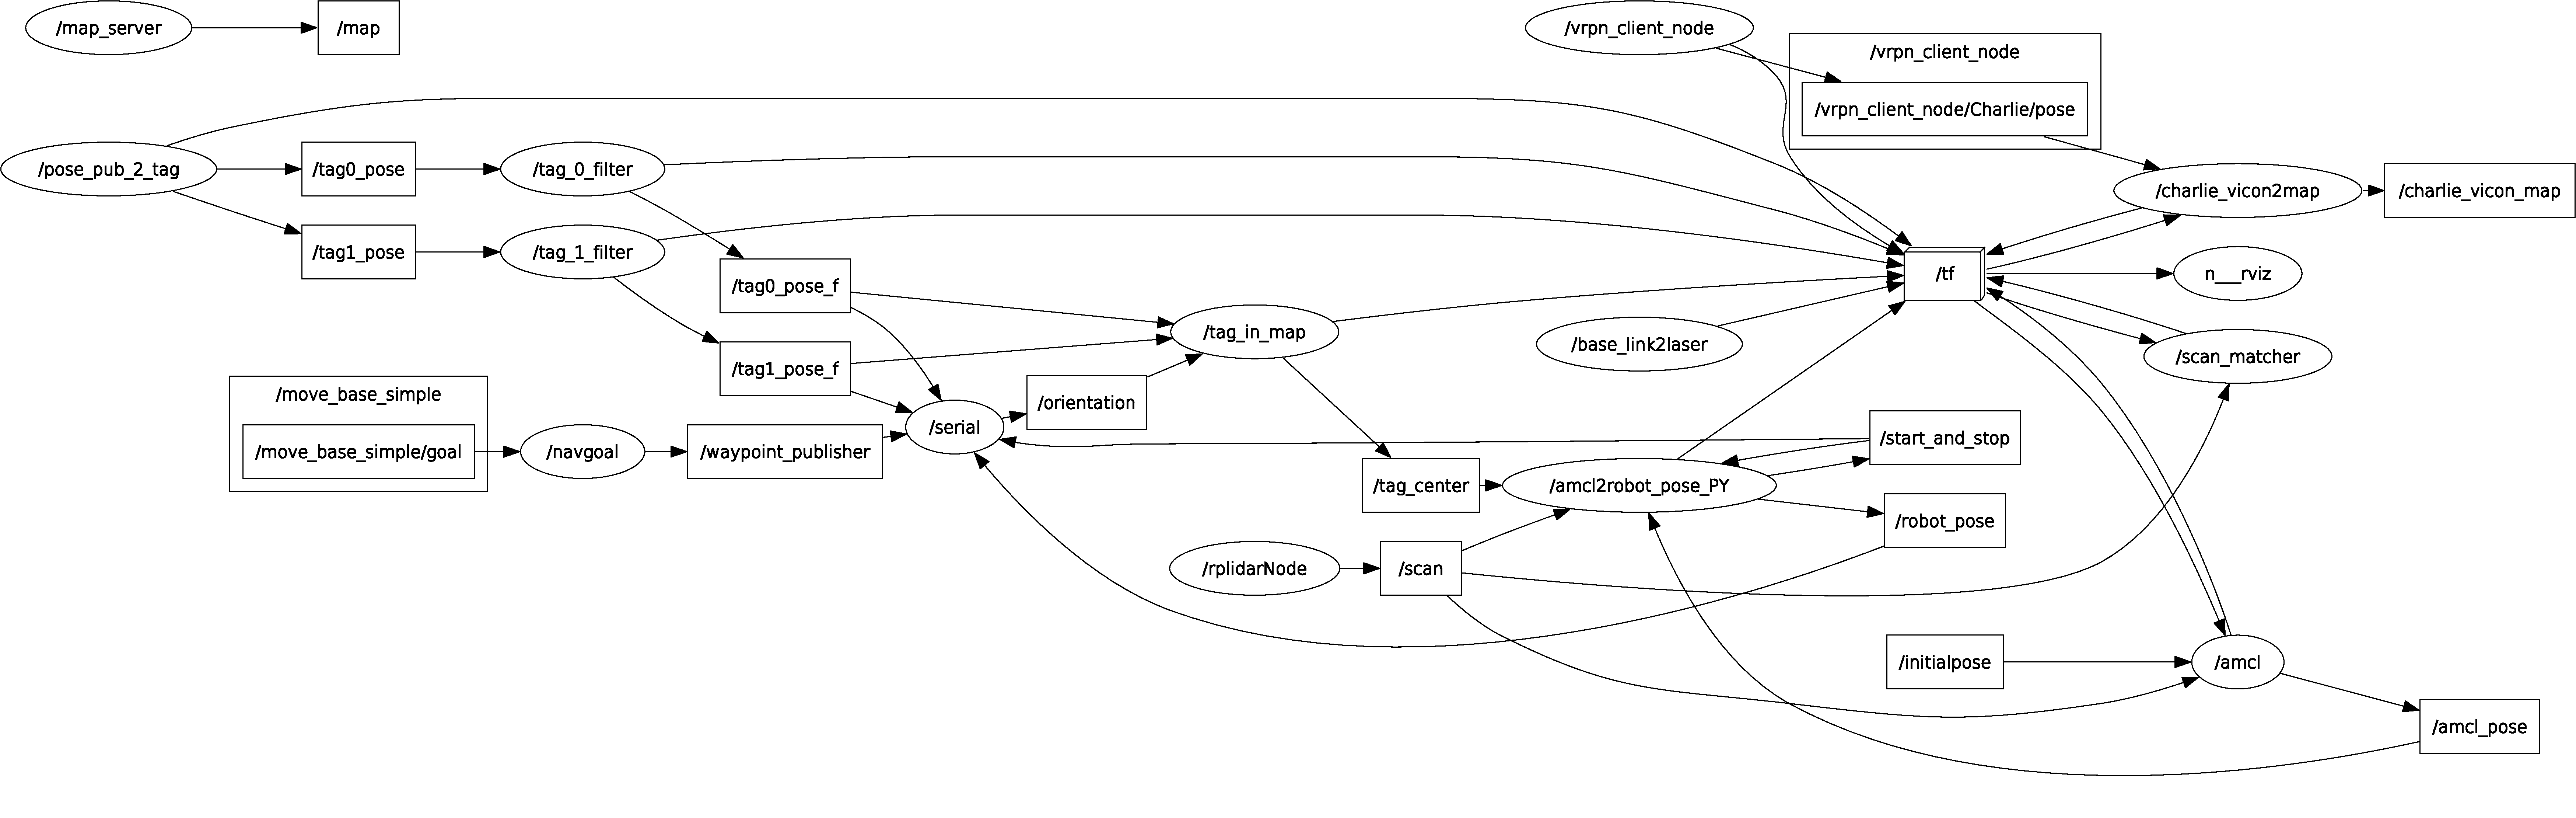
\includegraphics[width=\linewidth]{nodes_withtf_tree.pdf}
	\caption{Albero dei nodi}
	\label{fig: rqt_graph}
\end{figure}

\begin{figure}[h]
	\centering
	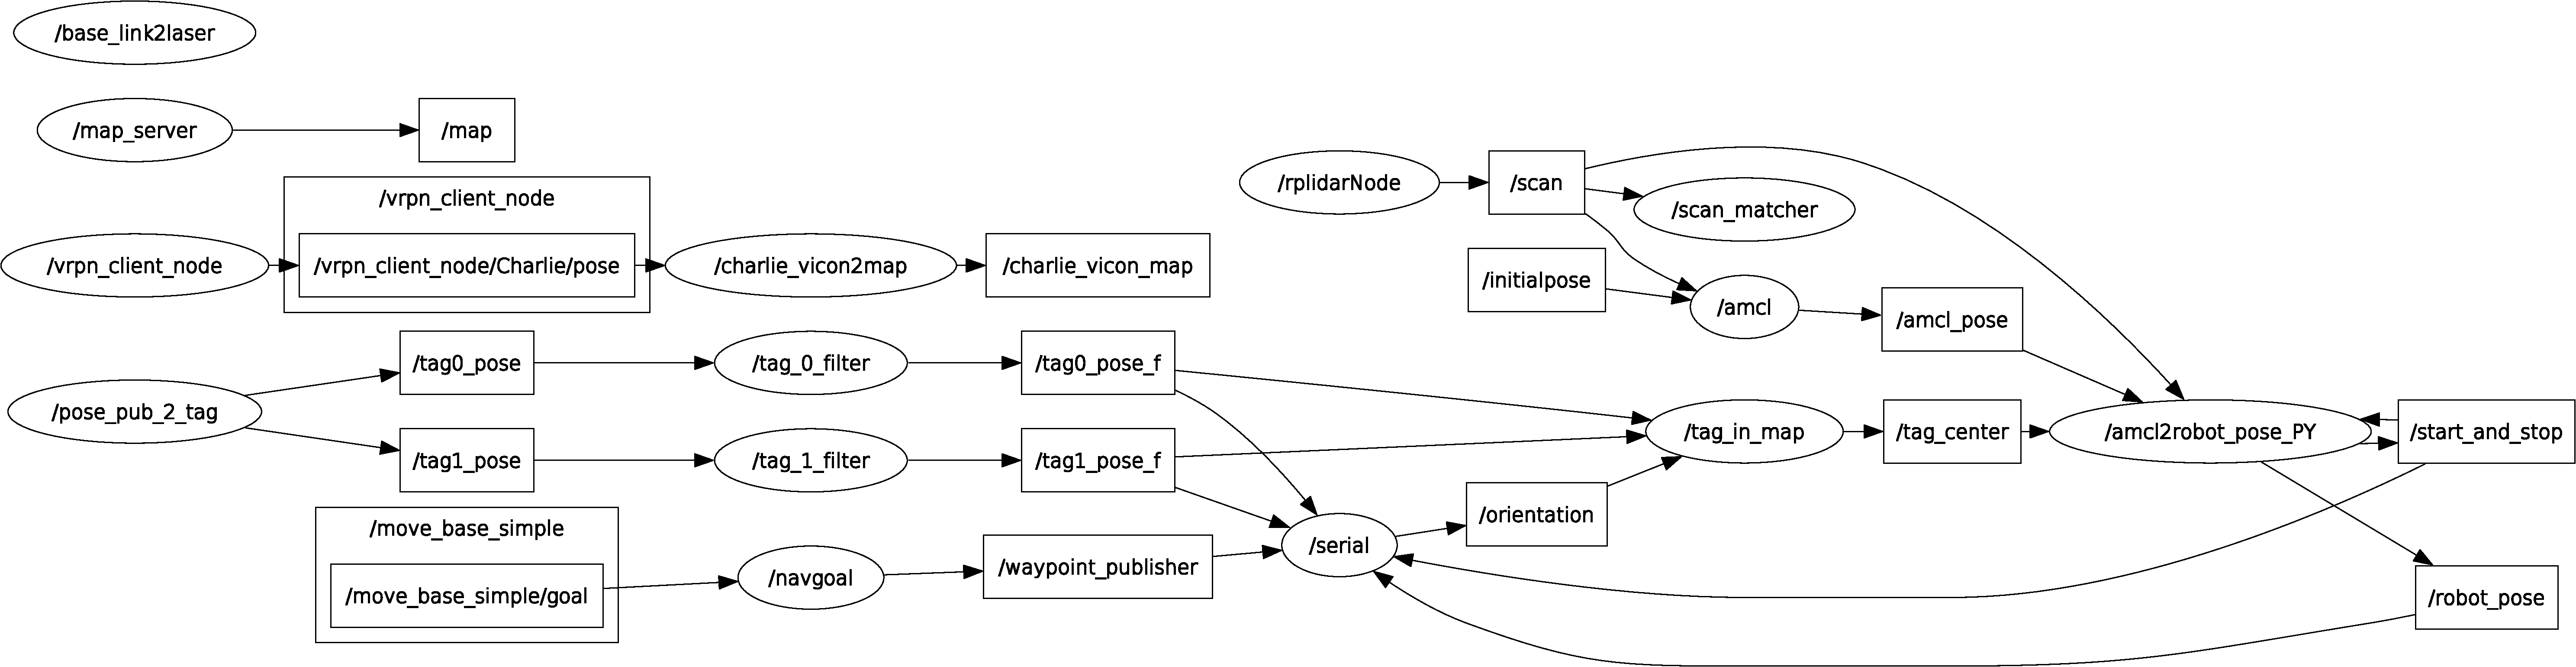
\includegraphics[width=\linewidth]{nodes_tree.pdf}
	\caption{Albero dei nodi, senza il topic \texttt{/tf}.}
	\label{fig: rqt_graph no tf}
\end{figure}



Seguendo fig.~\ref{fig: rqt_graph} da sinistra a destra e dall'alto verso il basso, adesso parleremo dei nodi (gli ellissi) e dei topic (i rettangoli) essenziali all'esperimento.
Per una maggiore immediatezza \`e possibile seguire il grafico di fig.~\ref{fig: rqt_graph no tf} in cui \`e stato omesso il topic \verb|/tf| ma questa non ha lo stesso ordine con cui stiamo per scrivere.

\vspace{0.5mm}
Il nodo \verb|/map_server| legge la mappa precedentemente acquisita e salvata con i comandi esposti in sez.~\ref{sez: nuova mappa} e la pubblica nell'omonimo topic: \verb|/map|.

Il cuore pulsante del sistema Pozyx \`e sicuramente racchiuso in \verb|/pose_pub_2_tag|. In questo si avvia la comunicazione con le due tag connesse via usb alla Raspberry, si salvano le coordinate delle ancore e quindi si esegue il posizionamento. 
Una volta fatto ci\`o si trasmettono le trasformazioni dei due tag sul topic \verb|/tf| e si pubblicano le loro pose sui rispetti topic: \verb|/tag0_pose| e \verb|/tag1_pose|.
Questi topic sono letti dai nodi \verb|/tag_0_filter| e \verb|/tag_1_filter| che ne fanno una media mobile a 10 campioni e la pubblicano su \verb|/tag0_pose_f| e su \verb|/tag1_pose_f|.

\vspace{0.5mm}
Facente parte dello stack di navigazione troviamo anche il topic \verb|/move_base_simple/goal| che rappresenta la posa desiderata in cui vogliamo che Charlie arrivi. 
Tale posa viene tradotta da \verb|/navgoal| in un messaggio \textit{Point} contenente $[x_{des}, y_{des}, \psi_{des}]$, in cui $\psi$ rappresenta l'heading angle desiderato, e pubblicato sul topic \verb|/waypoint_publisher|.

\vspace{0.5mm}
Di fondamentale importanza \`e il nodo \verb|/serial|. Questo infatti si occupa di comunicare alla STM la posizione filtrata dei tag, della posa attuale del robot (\verb|/robot_pose|) e l'avvio dei motori (\verb|/start_and_stop|). 
Inoltre dalla STM riceve l'angolo heading, ottenuto filtrando ulteriormente la posizione dei due tag, e lo pubblica in \verb|/orientation|.

Pi\`u nel dettaglio, l'STM32 sulla base dei dati ricevuti, calcola il controllo da dare ai motori per raggiungere l’obiettivo impostato; parallelamente a ciò calcola l'heading del veicolo tramite la posizione ricevuta dei due tag (\textit{attenzione}: il modello Simulink caricato sulla STM32 ha asse $Z$ rivolto verso il basso!).
I dati scambiati sono riassunti nelle tabelle~\ref{tab: comunicazione_seriale2stm}~e~\ref{tab: comunicazione_stm2seriale}.

\begin{table}[h]
		\centering
		\label{tab: comunicazione_seriale2stm}
		\begin{tabular}{lll}
			Nome                 & Descrizione                                & Dimensione\\
			\hline
			\verb!HEADER_A!      & 0x1A                                       & 1 Byte\\
			\verb!HEADER_B!      & 0x1B                                       & 1 Byte\\
			\verb!PAYLOAD!       & 0x2C                                       & 1 Byte\\
			\hline
			\verb!pos_x_f!       & tag $0$ - coordinata $x$ - frame UWB       & 4 Byte\\
			\verb!pos_y_f!       & tag $0$ - coordinata $y$ - frame UWB       & 4 Byte\\
			\verb!pos_z_f!       & tag $0$ - coordinata $z$ - frame UWB       & 4 Byte\\
			\hline
			\verb!pos_x_b!       & tag $1$ - coordinata $x$                   & 4 Byte\\
			\verb!pos_y_b!       & tag $1$ - coordinata $y$                   & 4 Byte\\
			\verb!pos_z_b!       & tag $1$ - coordinata $z$                   & 4 Byte\\
			\hline
			\verb!way_x!         & waypoint - coordinata $x$ - frame map    & 4 Byte\\
			\verb!way_y!         & waypoint - coordinata $y$ - frame map    & 4 Byte\\
			\verb!way_z!         & waypoint - $\psi$  - frame map            & 4 Byte\\
			\hline
			\verb!start_stop!    & $0$ = \textit{disabilita motori} $| 1$ =\textit{ abilita motori }      & 4 Byte\\
			\hline
			\verb!robot_pose_x!  & posa stimata da AMCL - coordinata x - frame map   & 4 Byte\\
			\verb!robot_pose_y!  & posa stimata da AMCL - coordinata y - frame map   & 4 Byte\\
			\verb!robot_pose_z!  & posa stimata da AMCL - $\psi$ - frame map            & 4 Byte\\
		\end{tabular}
		\caption{Comunicazione seriale \texttt{ttyUSBserial} Raspberry $\rightarrow$ STM32}
\end{table}


I primi tre elementi sono header che codificano il tipo di messaggio, mentre i restanti sono informazioni utili che verranno lette ed interpretate. 

In dettaglio, le coordinate delle due tag vengono utilizzate dall'STM per misurare l'heading del veicolo\footnote{L'angolo è misurato rispetto all'asse $x$ del frame \texttt{UWB}, riportandolo poi in un sistema di riferimento $z-down$}, che insieme alla posa stimata da AMCL, ed al waypoint impostato, sono sfruttate per determinare il controllo dei motori. Infine l'elemento \verb!start_stop! (booleano) li abilita o disabilita.
Il valore di $\psi$ è inviato dall'STM in un pacchetto come quello mostrato in Tabella~\ref{tab: comunicazione_stm2seriale}.

\begin{table}[h]
	\centering
	\label{tab: comunicazione_stm2seriale}
	\begin{tabular}{lll}
		\hline
		Nome                     & Descrizione   & Dimensione\\
		\hline
		\verb!HEADER_A!          & 0x1A          & 1 Byte\\
		\verb!HEADER_B!          & 0x1B          & 1 Byte\\
		\verb!PAYLOAD_POSE!      & 0x2C          & 1 Byte\\
		\hline
		\verb!heading!           & $\psi$         & 4 Byte\\
		\hline
	\end{tabular}
	\caption{Comunicazione STM32 $\rightarrow$ \texttt{ttyUSBserial} Raspberry}
\end{table}

\vspace{0.5mm}
Riprendendo fig.~\ref{fig: rqt_graph} con il nodo \verb|/tag_in_map| questo \`e incaricato di tradurre la posa dei tag e di restituirla in coordinate espresse in map--frame. 
Di fatto effettua una media della posizione dei due tag, ci somma un vettore costante in frame body (ovvero l'offset tra centro e lato del veicolo) ruotato dell'angolo $\psi$ letto dal topic \verb|/orientation|.
Infine pubblica la trasformazione corrispondente in \verb|/tf| e in \verb|/tag_center|.

\vspace{0.5mm}
Il nodo \verb|/rplidarNode| creato da Slamtec si interfaccia, appunto, con il Lidar Slamtec. 
\`E in grado quindi di avviare o interrompere il motore del lidar, di comunicare via seriale le scansioni e infine di pubblicarle nel relativo topic \verb|/scan|.

\vspace{0.5mm}
Il blocco ad alto livello della localizzazione di Charlie \`e costituito principalmente dai nodi che si interfacciano con il topic \verb|/tf|, ossia: \verb|/scan_matcher|, \verb|/amcl| e \verb|/amcl2robot_pose_PY|.
I primi due confrontando la scansione pi\`u recente del lidar con le precedente e soprattutto con la mappa nota riescono a fornire una stima di odometria. Il terzo, \verb|/amcl2robot_pose_PY|, si occupa di fornire la posa stimata ad una maggiore frequenza rendendola cos\`i disponibile all'algoritmo di guida caricato sull'STM32.

\vspace{0.5mm}
Infine, parallelamente ai nodi descritti finora si inserisce il sistema Vicon, utilizzato solamente come ground-truth all'algoritmo di localizzazione. 
Questo \`e composto da \verb|/vrpn_client_node| che comunicando con il server Vicon pubblica le pose degli oggetti selezionati (rifarsi a sez.~\ref{sez:Sistema Vicon}) sul topic corrispondente. 
La posa di Charlie, espressa in Vicon-frame viene tradotta sottoscrivendosi al topic \verb|/tf| nel frame \verb|/map| cos\`i da avere un rapido confronto a posteriori.


\subsubsection{Sistemi di riferimento}
\begin{figure}[h]
	\centering
	\includegraphics[height=0.3\textheight]{charlie_vista_alto.pdf}
	\caption{Charlie body frame.}
	\label{fig: charlie body frame}
\end{figure}

\begin{figure}[h]
	\centering
	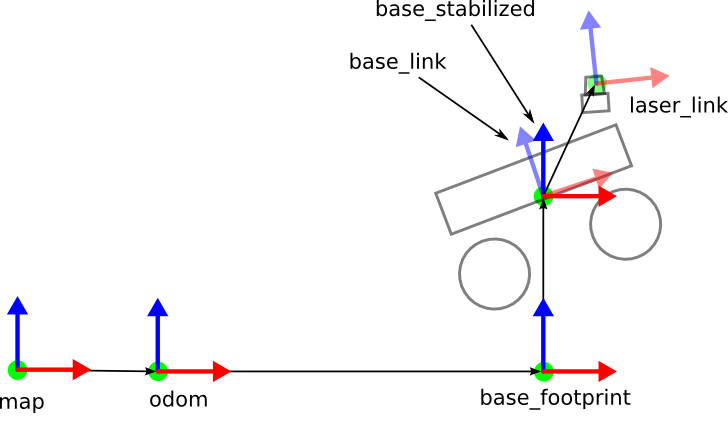
\includegraphics[height=0.25\textheight]{coordsystems_hector.png}
	\caption{Frame utilizzati dal navigation stack.}
	\label{fig: hector frames}
\end{figure}

I sistemi di riferimenti utilizzati sono quelli riportati nell'albero in fig.~\ref{fig: rqt_tf_tree}. 
Oltre a quelli gi\`a riportati nelle sezioni precedenti, c'\`e da sottolineare com'\`e stato scelto il sistema di riferimento body di Charlie e come i diversi sistemi di riferimento da \verb|base\_link| a \verb|laser| interagiscono.

Il primo ha l'asse $x$ nella direzione di avanzamento e l'asse $z$ \`e stato scelto coerente con gli assi $z$ del frame UWB e Vicon: con $z$ rivolto verso l'alto. Attenzione che l'STM32 utilizza la convezione $z$-down. Per quanto riguarda l'origine, come in fig.~\ref{fig: charlie body frame}, questa si trova nel centro del veicolo.

I vari frame utilizzati da \texttt{hector\_slam} e dal navigation stack sono visibili in fig.~\ref{fig: hector frames}. Per il nostro scopo i frame \texttt{odom}, \texttt{base\_footprint}, \texttt{base\_link} e \texttt{laser} sono tutti coincidenti.


\begin{figure}[]
	\centering
	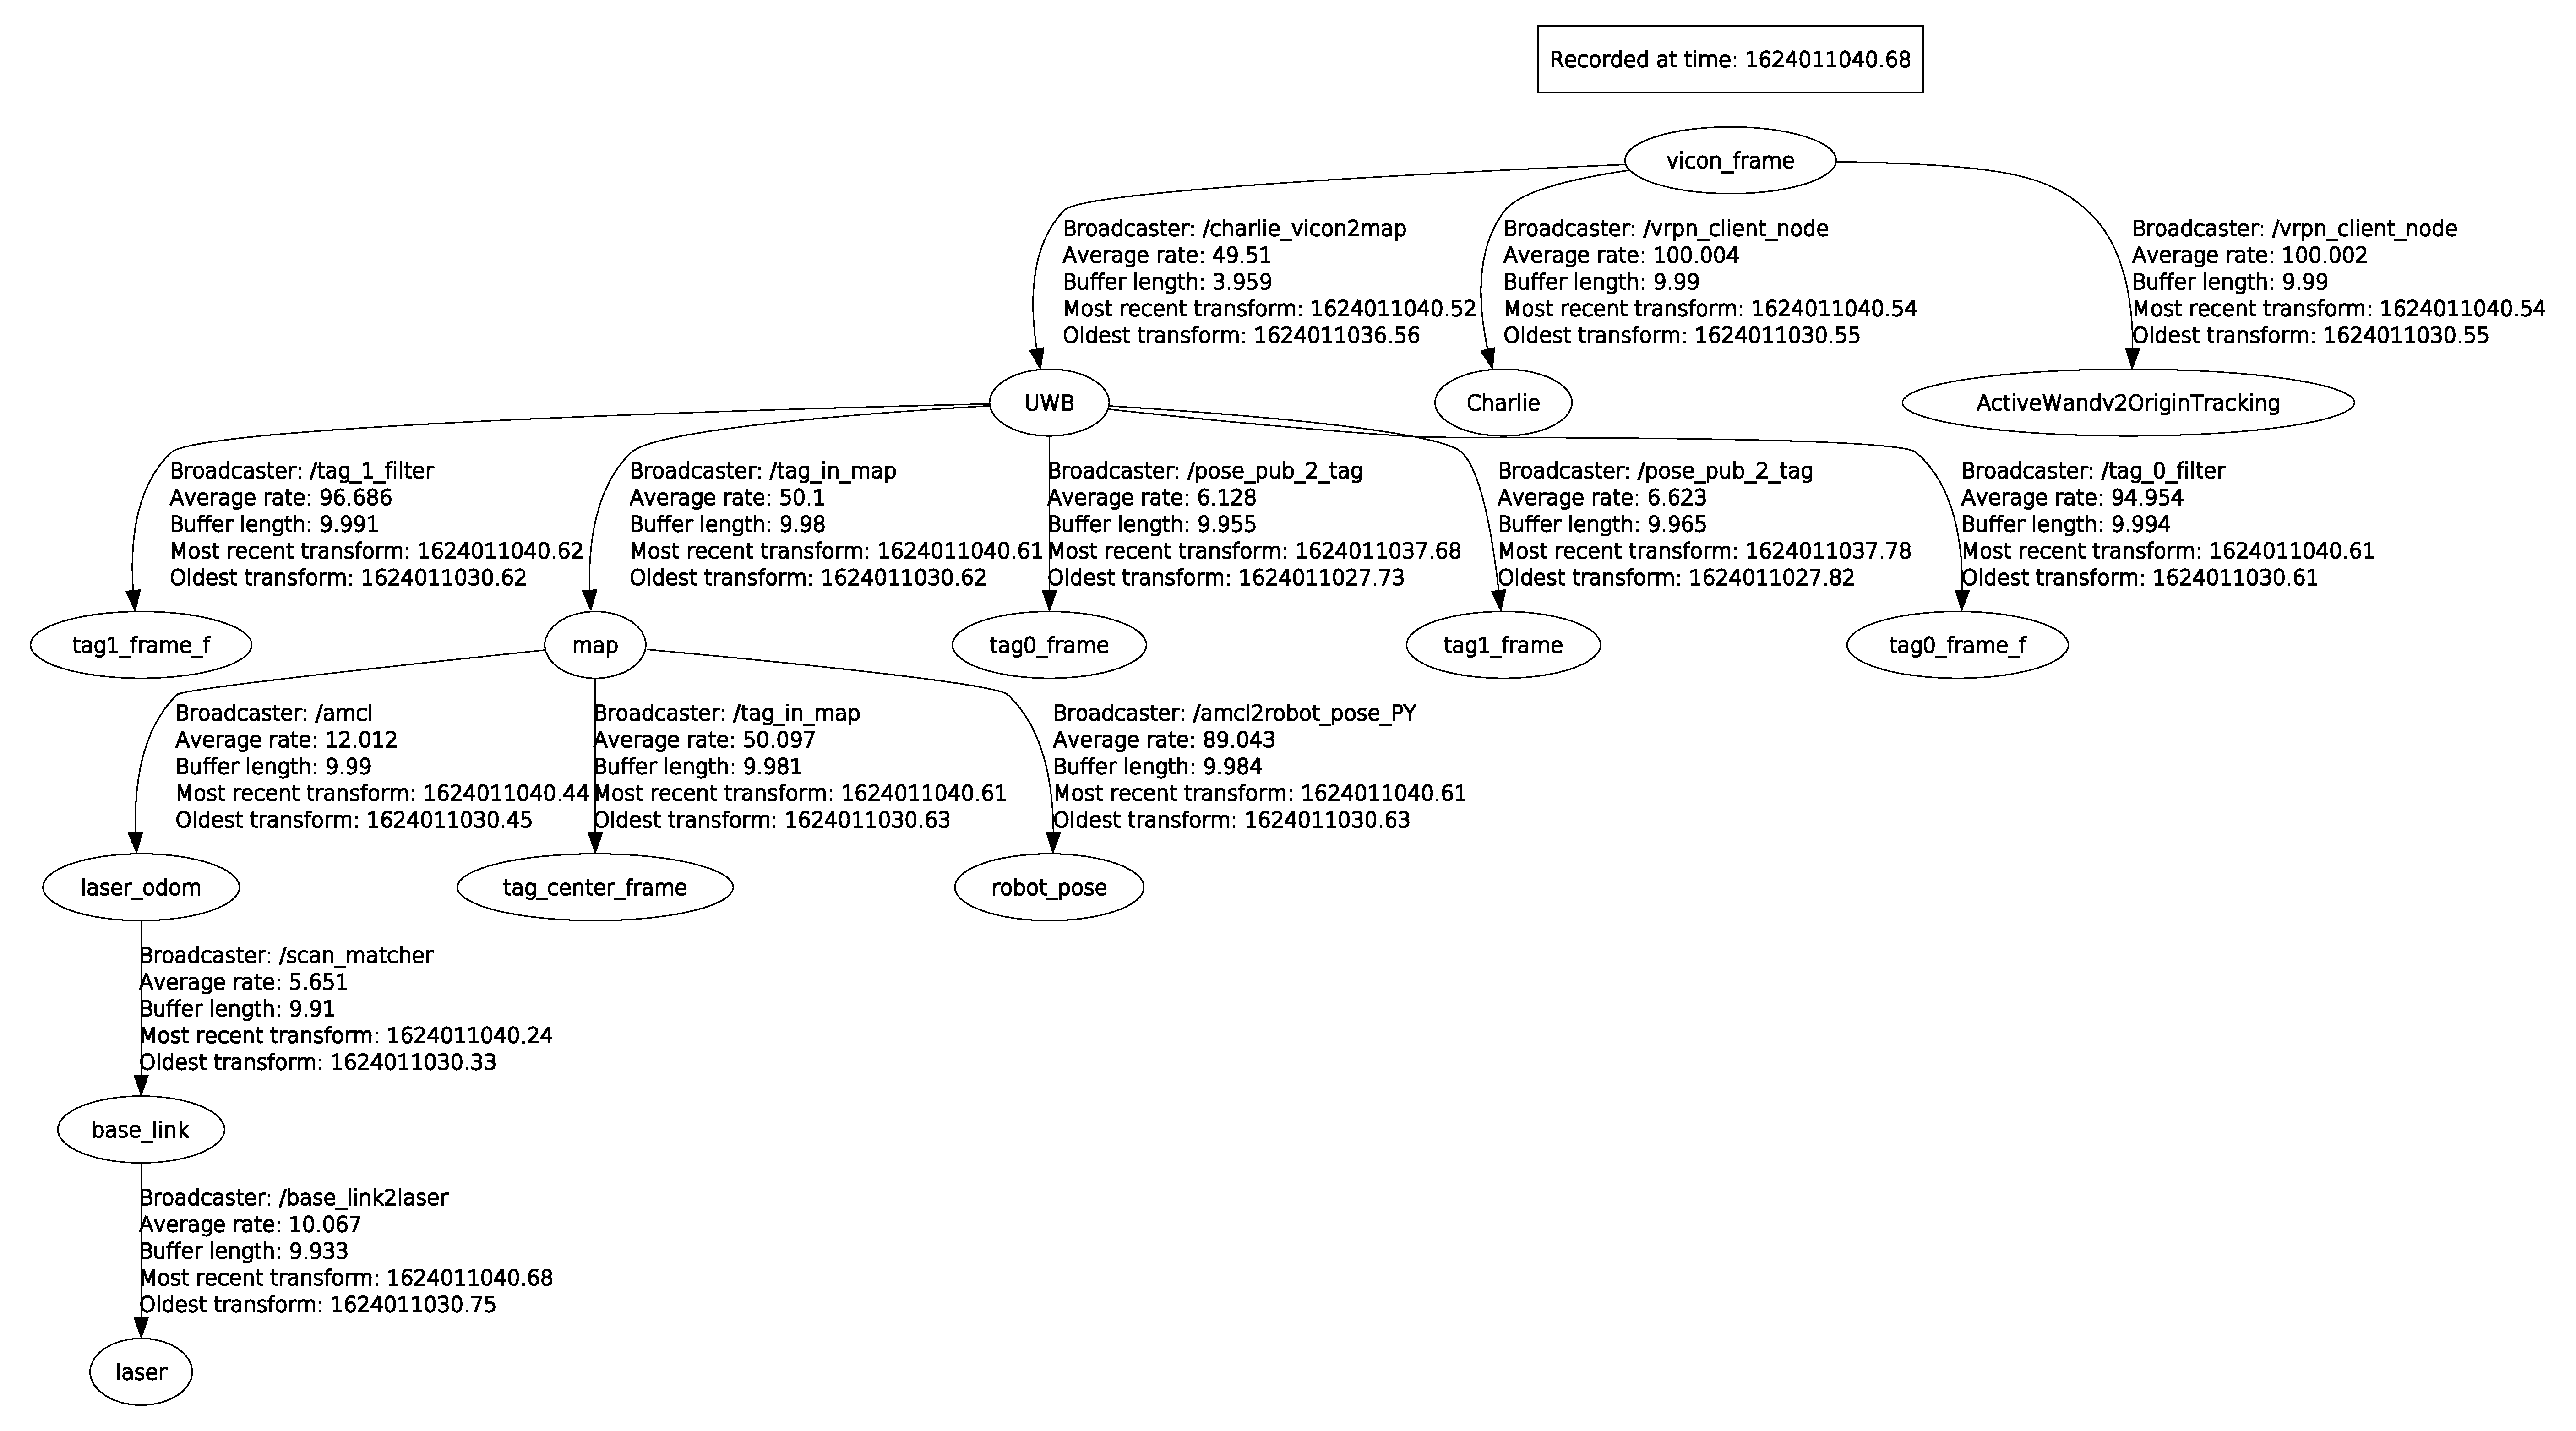
\includegraphics[width=\linewidth]{tf_tree.pdf}
	\caption{Albero delle trasformazioni}
	\label{fig: rqt_tf_tree}
\end{figure}

\FloatBarrier

%%%%%%%%%%%%%%%%%%%%%%%%%%%%%%%%%%%%%%%%%%%%%%%%%%%%%%%%%%%%%%%%%%%%%%%%%%%%%%%%%%%%%%%%%%%%%%%%%%%%%%
\newpage
\section{Esperimenti}

Una volta terminato il porting del sistema sulla scheda RaspberryPi4, corredate da modifiche nel codice pre esistente (dove necessario),
abbiamo pensato alcuni scenari per testare la bontà del sistema nello stato attuale. Per quanto riguarda l'impostazione di prove pensate
per una verifica del buon funzionamento delle procedure di fix di posa e dell'algoritmo di navigazione, anche su più stanze, rimandiamo agli 
esperimenti e ai risultati riportati nella relazione precedente, ovvero \cite{ptvlocalizzazione}, dato che non sono state apportate modifiche
alla loro struttura durante il nostro lavoro. 
Nel nostro caso, la verifica della navigazione con AMCL è stata impostata sfruttando la presenza del sistema Vicon.
Per evidenziare al meglio il nostro ruolo e contributo nello sviluppo di questo sistema, è stato deciso di orientare l'analisi verso due obiettivi
specifici: il primo è quello di portare un'analisi più dettagliata degli errori compiuti dal sistema durante la localizzazione con UWB, dove 
auspichiamo che alcune modifiche e accorgimenti possano portare ad una riduzione degli errori che ha presentato fino ad ora (tali da escludere il 
sistema UWB dall'essere il mezzo primario di navigazione e circoscrivere il suo ruolo a quello del fix di posa in caso di fallimento del lidar, 
sensore protagonista della navigazione). 
Per farlo, abbiamo utilizzato come ground-truth il sistema Vicon, disponibile però solo nella stanza del volo e, per questo motivo, di limitata 
ripetibilità pratica. Abbiamo deciso comunque di riportarne i risultati, in modo da fornire un riferimento affidabile di quelli che sono gli errori
compiuti, per i quali ci aspettiamo una somiglianza in tutte le configurazioni simili a quella ricreabile nella stanza del volo stessa (ambiente
chiuso, presenza di finestre, estensione non troppo elevata, assenza di ostacoli all'interno dell'area di moto). Tale confronto è stato fatto 
sia in termini di posizioni statiche delle ancore, andando così a valutare la bontà della procedura di autocalibrazione, sia riguardo la posa 
dinamica (posizione e assetto) assunta da Charlie quando si muove nello spazio e viene localizzato dal solo sistema UWB.
Sempre sfruttando la presenza del Vicon, abbiamo successivamente deciso di effettuare un esperimento classico, vedere \ref{sez: Guida breve all'esperimento}, 
ovvero attivando la navigazione con l'STM (AMCL e Lidar adesso sono attivi), fatta però con il Vicon acceso in modo da avere un ground truth sulla effettiva
posa di Charlie. Per questa prova, non è stato utilizzata una guida manuale, bensì attraverso comandi dati da \verb|Rviz| attraverso il comando \verb|2DNavGoal|, 
che permette di dire al veicolo in quale punto della mappa spostarsi e con quale orientazione.

Viste le modifiche effettuate sul sistema UWB per quanto concerne la procedura di salvataggio delle pose delle ancore a fine autocalibrazione, 
abbiamo predisposto una prova in esterno per valutare eventuali migliorie di funzionamento. Il sistema UWB si trova in questo caso in un ambiente 
favorevole rispetto a quando è utilizzato indoor. In particolar modo, andremo a testarne il funzionamento in un cortile interno al polo A di 
Ingegneria, dove ci aspettiamo diversi disturbi per le UWB, legati alla presenza di molti oggetti e strutture metalliche (tra cui la rampa di 
scale di emergenza) e di finestre poste in line of sight con le ancore stesse.
Essendo l'estensione del cortile maggiore rispetto a quella della stanza del volo, ciò ci consentirà anche di valutare il raggio di azione di 
questo sistema e, di controparte, la difficoltà che può riscontrare il lidar quando si trova in assenza di riferimenti fissi abbastanza vicini, 
come pareti, per l'acquisizione dei suoi dati.

\subsection{Confronto UWB e Vicon: posizione antenne}

\begin{figure}
	\centering
	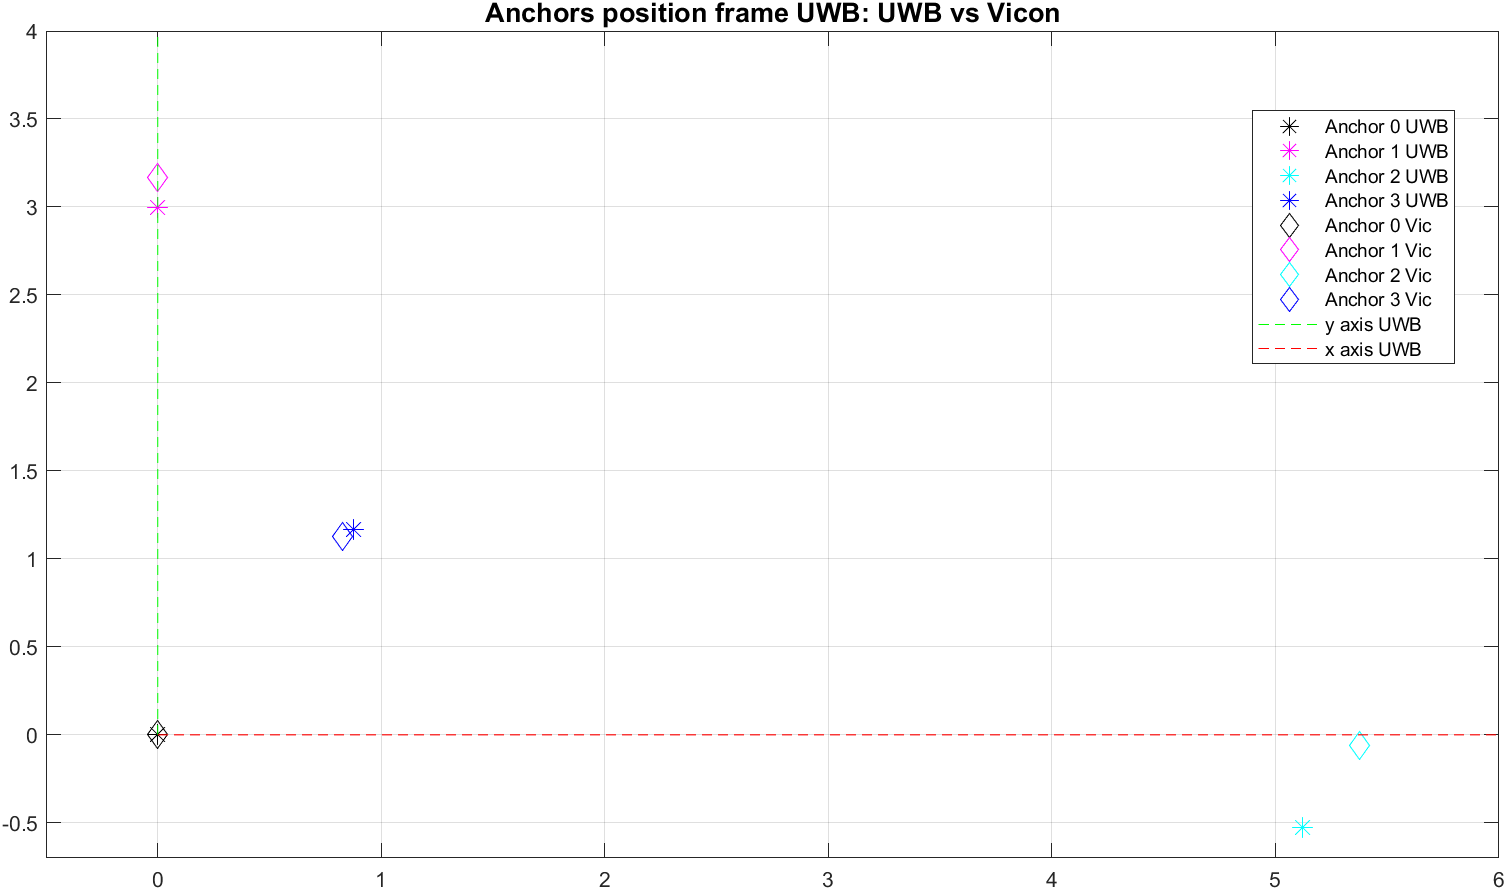
\includegraphics[height=0.4\textheight]{anchors_UWB_Vicon.png}
	\caption{ancore in UWB frame: UWB vs Vicon}
	\label{fig: ancore in UWB frame, UWB vs Vicon}
\end{figure}

La prima prova che abbiamo deciso di effettuare è stata quella volta alla valutazione dell'affidabilità della procedura di autocalibrazione delle ancore del
sistema Pozyx. Durante il nostro lavoro, infatti, erano state riscontrate alcune anomalie, corrette andando a modificare la gestione degli ID nell'esecuzione 
di alcune funzioni di \verb|positioning| del sistema Pozyx, dove è necessario porre attenzione affinché chi è demandato di eseguirle, tra gli elementi del sistema, 
abbia al suo interno effettivamente tutte le informazioni corrette e aggiornate di cui necessita. Per questo motivo, abbiamo agito sulla procedura di salvataggio 
facendo in modo che sia garantita la presenza all'interno della memoria dei chip delle ancore l'informazione della propria posizione a valle dell'ultima 
utocalibrazione. 
Per validare la bontà dell'autocalibrazione, che viene eseguita seguendo la procedura descritta in sez.~\ref{sez:Autocalibrazione}, si sfrutta come ground truth il 
Vicon, in questo caso affiancato alla Wand, una sorta di struttura a forma di croce, sulla quale sono fissati dei marker con configurazione asimmetrica e il cui 
rispettivo oggetto virtuale è già preimpostato sul sw per la gestione del Vicon. 
Quest'ultimo sarà necessario per andare ad individuare la posizione delle ancore, prive di marker riconoscibili dal Vicon. Tali misure, da considerarsi prive di 
errori legati allo strumento, ma affette da errori dovuti al posizionamento della Wand sulle ancore stesse (errore umano di esecuzione), verranno confrontati con 
quelli ottenuti a valle del procedimento di autocalibrazione, dove in uscita ogni ancora è a conoscienza della propria posizione espressa rispetto al sistema di 
riferimento costruito su di esse (\verb|UWB frame|).

Le ancore sono state poste in una configurazione che a nostro avviso, dopo aver fatto varie prove, è quella che permette di ottenere una autocalibrazione più corretta: 
troviamo le prime tre ancore alla stessa altezza e messe in modo da delimitare gli assi x, y e l'origine, mentre la quarta ancora è alzata molto lungo la verticale 
e posta nei pressi dell'origine (riferirsi alla fig.~\ref{fig: disposizione ancore}). Nel caso in cui questa venga allontanata troppo, l'algoritmo di autocalibrazione 
fallisce (si hanno problemi di radici di numeri negativi nella parte algebrica).

Come descritto in \ref{sez: Guida breve all'esperimento}, per questo primo test andremo a:
\begin{itemize}
	\item Avviare i dialoghi tra ros e il sistema Vicon, eseguendo da pc il file di lancio \verb|vicon_charlie.launch|.
	\item Salvare la trasformazione tra Vicon e UWB eseguendo il file \verb|vicon2uwb_tf.py|. In questa fase, sarà richiesto di posizionare sequenzialmente la Wand 
	in corrispondenza dell'ancora 0, poi dell'ancora 1 e così via. Per ciascun posizionamento, premendo \verb|Enter| da tastiera si andrà a salvare la posizione, in 
	frame Vicon, della Wand in quell'istante, coincidente con quella dell'ancora sulla quale è posizionata. In questo modo, vengono salvate le coordinate delle 4 ancore in frame \verb|Vicon frame|.
	\item Sempre all'interno di \verb|vicon2uwb_tf.py|, tali posizioni vengono riportate ad essere espresse nel sistema di riferimento UWB, ovvero \verb|UWB frame|, 
	in quanto la loro posizione a seguito dell'autocalibrazione è nota nel sistema di riferimento \verb|UWB|.
\end{itemize}

Sono riportate di seguito le due misure:

Ancore misurate con UWB (a seguito della procedura di autocalibrazione), riportate in \SI{}{\metre}
\begin{itemize}
	\item Anchor 0, 0x6902 $\rightarrow$ X: 0.0, 	Y: 0.0, 	Z: 0.0
	\item Anchor 1, 0x6e7a $\rightarrow$ X: 0.0, 	Y: 2.997, 	Z: 0.0
	\item Anchor 2, 0x6e44 $\rightarrow$ X: 5.121, Y: -0.527, 	Z: 0.0
	\item Anchor 3, 0x6e6c $\rightarrow$ X: 0.875,	Y: 1.165, 	Z: 1.295
\end{itemize}

Ancore misurate con Vicon (riportate in \verb|UWB frame|) espresse in \SI{}{\metre}
\begin{itemize}
	\item Anchor 0, 0x6902 $\rightarrow$ X: 0.000000,	Y: 0.000000,	Z: 0.000000
	\item Anchor 1, 0x6e7a $\rightarrow$ X: 0.000000,	Y: 3.168643,	Z: 0.032111
	\item Anchor 2, 0x6e44 $\rightarrow$ X: 5.378095,	Y: -0.063190,	Z: -0.047064
	\item Anchor 3, 0x6e6c $\rightarrow$ X: 0.826354,	Y: 1.129845,	Z: 1.239518
\end{itemize}


Come possiamo osservare dai risultati ottenuti, graficati in fig.~\ref{fig: ancore in UWB frame, UWB vs Vicon}, troviamo un errore di almeno \SI{20}{\centi \metre} sulle coordinate delle varie ancore, che però sembra non raggiungere valori troppo elevati, se non nel caso della coordinata Y della terza ancora, dove l'errore è di circa 
\SI{45}{\centi \metre}. Siamo piuttosto soddisfatti di questo risultato in quanto anche dai precedenti esperimenti era nota la presenza di un errore sistematico legato alle 
UWB, dovuto probabilmente a limiti del metodo stesso più che ad errori nell'algoritmo scritto: l'ambiente indoor e l'utilizzo di sole 4 ancore non permette di ottenere
misure precise nello spazio 3D, dove dalla documentazione ufficiale della Pozyx si legge che sarebbero necessarie almeno 6 ancore poste ad altezze diverse tra di loro 
per raggiungere migliori performance in termini di riduzione dell'errore.                                                  

\subsection{Confronto UWB e Vicon: Charlie}

Come per la prima prova, anche la seconda vede l'utilizzo del Vicon come ground truth e per questo è stata eseguita all'interno della stanza del volo del polo A.
Come prima cosa, è necessario posizionare dei marker sul veicolo in modo asimmetrico. Nel nostro caso sono stati posizionati come in fig.~(FAI RIF), dove vediamo 
marker: uno centrato nella parte frontale, due laterali a circa metà della struttura e un quarto nella parte posteriore, spostato verso destra per ottenere 
l'asimmetria necessaria ad evitare ambiguità. Il sistema Vicon riesce con essi a costruire un oggetto virtuale corrispondente a Charlie senza ambiguità di orientazione. 
Una volta costruito tale oggetto, per il procedimento riferirsi al \ref{sez:Sistema Vicon_oggetto}, si può procedere con l'esperimento vero e proprio. In questo caso, 
per i comandi di spostamento è stato utilizzato il radiocomando, così da avere maggiore manovrabilità.

Dato che, in questa prova, il nostro interesse principale verte sulla valutazione della bontà del sistema UWB per la localizzazione, non andiamo ad utilizzare il file
di lancio adibito alla navigazione con Lidar e AMCL (\verb|localization.launch|), dove UWB entra in gioco solo nel momento in cui la posa data dal Lidar con AMCL differisce di più di \SI{1.5}{\metre}| da quella data dal sistema UWB, come descritto e analizzato in \cite{ptvlocalizzazione} nei primi due esperimenti riportati. 
 
Abbiamo deciso quindi di limitarci alla localizzazione effettuata con le UWB: per farlo, sarà sufficiente avviare la localizzazione delle tag con il sistema di 
ancore tramite il comando:
\begin{verbatim}
	roslaunch charlie_launch start_uwb.launch		# avvia uwb
\end{verbatim} 

Una volta fatto ciò, si passa al lancio del sistema di acquisizione dati del Vicon, vedere \ref{sez:Sistema Vicon}, dopo aver aggiunto i topic relativi al Vicon
nella lista di quelli da registrare nella bag. 
Avviati tutti i nodi ros necessari, si può procedere semplicemente spostando Charlie nella stanza, raccogliendo così le medesime informazioni in due modi distinti: 
uno (il Vicon) considerato corretto e privo di errori, l'altro (il sistema UWB), affetto da errori che vogliamo individuare.

Si procede, quindi, all'analisi dei dati attraverso Matlab. Il codice relativo si trova nel file
\begin{verbatim}
	...\Analisi_matlab\Analisi_uwbvicon_confronto.m
\end{verbatim}  
Abbiamo per prima cosa confrontato i dati grezzi delle posizioni \verb|x| e \verb|y| delle due tag (tag0 e tag1) misurate dal Vicon e dal sistema UWB, di quest'ultimo 
riportandone sia la misura ``raw'' sia quella filtrata con un filtro a media mobile, come vediamo in fig.~\ref{...}.

In collegamento a questi ultimi, abbiamo anche graficato l'errore commesso da UWB nel restituire tali coordinate.
Sempre riguardo all'errore per le due tag, abbiamo visualizzato il vettore errore normalizzato rispetto alla circonferenza unitaria centrata nell'origine, così da 
renderci conto se esiste una significativa direzionalità di questo errore o se, invece, esso assume orientazioni casuali distribuendosi uniformemente sulla 
circonferenza di riferimento: possiamo subito notare che, per entrambe le tag, l'errore si distribuisce molto di più nei quadranti negativi della circonderenza,
mentre in quelli positivi si contano solo pochi campioni isolati.

\textbf{PLOT QUIVER DIRE}

Similmente, considerando che dalla posizione delle due tag su Charlie è possibile ricavare l'heading del veicolo, abbiamo deciso di confrontare l'heading calcolato
come \verb|atan2| tra le posizioni ricavate con UWB, con quello fornitoci direttamente dal Vicon (ritenuto il ground truth) e con quello che esce fuori dall'STM 
(legato alle uscite degli algoritmi di guida in esso integrati?????). Anche qua evidenziamo un errore sistematico nell'angolo, sicuramente legato anche al fatto 
che, a differenza di quanto possiamo aspettarci, il gap tra i due diminuisce, e di conseguenza diminuisce anche l'errore in heading, mentre nei momenti in cui 
l'assetto pare essere costante torna a vedersi in modo chiaro l'offset iniziale, che non viene mai recuperato.

Può inoltre essere interessante andare a distinguere le varie fasi di moto di Charlie, ovvero i punti in cui sta fermo, quelli in cui procede in linea retta e 
quelli dove, invece, compie traiettorie curvilinee, ed associare ad essi i pattern seguiti dai vari errori: come ci aspettiamo, la fase in cui l'errore si riduce 
maggiormente coincide con quella in cui Charlie sta fermo (da \SI{50}{\second} a \SI{60}{\second}). Questo non accade però, come già accennato, per quanto riguarda l'heading, 
dove a causa di un offset iniziale pare esserci un maggiore errore quando l'angolo non varia rispetto ai momenti in cui si riorienta.

\textbf{valutazione dei risultati di questa prima prova con i vari grafici}

Dai risultati ottenuti, abbiamo riscontrato un'errore sbilanciato verso la parte negativa, che aumenta soprattutto nelle fasi di moto. Per valutare se c'è un'influenza 
dell'autocalibrazione e del modo in cui sono state posizionate le ancore, abbiamo deciso di ripetere un secondo esperimento cambiando l'assetto del sistema. La prima modifica è stata quella di posizionare le ancore con una differenza di altezza maggiore, in modo da consentirci 
di distanziare maggiormente la quarta ancora dall'origine senza che ciò generi errori nella creazione del frame UWB (durante la procedura di autocalibrazione, 
descritta in \ref{sez:Autocalibrazione}). Per ricreare una configurazione il più possibile favorevole per l'ottenimento un buon setting, abbiamo messo le ancore 
a formare una figura che si avvicini ad un tetraedro, configurazione più adatta per ottenere una buona autocalibrazione.
Parallelamente a questo cambiamento, abbiamo deciso di valutare anche la possibilità di variare la posizione relativa tra le ancore, montate sui supporti, e 
le powerbank utilizzate per alimentarle: fino ad ora queste erano appoggiate esattamente al di sopra delle strutture delle rispettive ancore. In questo modo, 
però, si incorre nel rischio di creare forti disturbi al sistema, in quanto l'antenna presente sulle ancore punta proprio verso l'alto, dove si trova la powerbank. 
Per cercare di limitare i disturbi, abbiamo deciso di fissarle al di sotto della struttura e di ripetere la prova in questa nuova configurazione.

\textbf{FINIREEEEEEE E ANALIZZARE I GRAFICI E RIPORTARLI }

\subsection{Navigazione Charlie con AMCL e Vicon come ground truth}

Qua si tratta di un esperimento standard (vedere \ref{sez: Guida breve all'esperimento}), dove in parallelo alla navigazione gestita attraverso l'algoritmo AMCL, viene attivato anche il ``motion capture''
di Charlie attraverso il sistema Vicon. Questo permette di avere un ground truth sulla posizione e l'orientazione del veicolo durante la navigazione compiuta
nell'ambiente sfruttando l'algoritmo di AMCL. In questo modo, siamo in grado di fornire un riferimento di quello che effettivamente è l'errore di navigazione compiuto dal sistema e, nel caso appaiano errori sistematici, di individuarli e poterne indagare la causa.
La nostra preoccupazione qua non è stata, come detto nell'introduzione della sezione, quella di verificare il funzionamento del fix di posa dell'algoritmo di navigazione, bensì quello di valutare l'errore che viene fatto con AMCL e con le sole UWB rispetto ad un ground-truth affidabile, quale il Vicon, durante un esperimento standard. Per questo motivo, non sono state salvate nella bag le informazioni pubblicate nel topic \verb|\initialpose|, così come non abbiamo riportato le pose delle singole tag, bensì direttamente quella associata al centro del sistema di riferimento solidale al veicolo.
Nello specifico, i topic salvati per questo esperimento sono:
\begin{verbatim}
	%	rosbag info 'Confronto_stanzavolo_Vicon.bag'
	
	/amcl_pose			% posa di Charlie data da AMCL e espressa in map frame 
	/charlie_vicon_map	% posa di Charlie registrata da vicon e riportata in map frame
	/map
	/orientation
	/particlecloud
	/robot_pose			% posa di Charlie data ZOH su quella derivante da AMCL (map frame)
	/rosout
	/rosout_agg
	/scan   
	/tag_center			% posa di Charlie misurata dal sistema UWB e riportata in map frame
	/tf     
	
\end{verbatim}

Con questi dati, abbiamo deciso di formulare la seguente analisi.
Come prima cosa, abbiamo verificato il tracciato registrato con 3 diversi metodi: Vicon, navigazione con AMCL e registrazione delle posizioni dal sistema Pozyx, come riportato in fig.~\ref{fig: traiettorie_vicon_charlie}

\begin{figure}[] 
	\centering    
	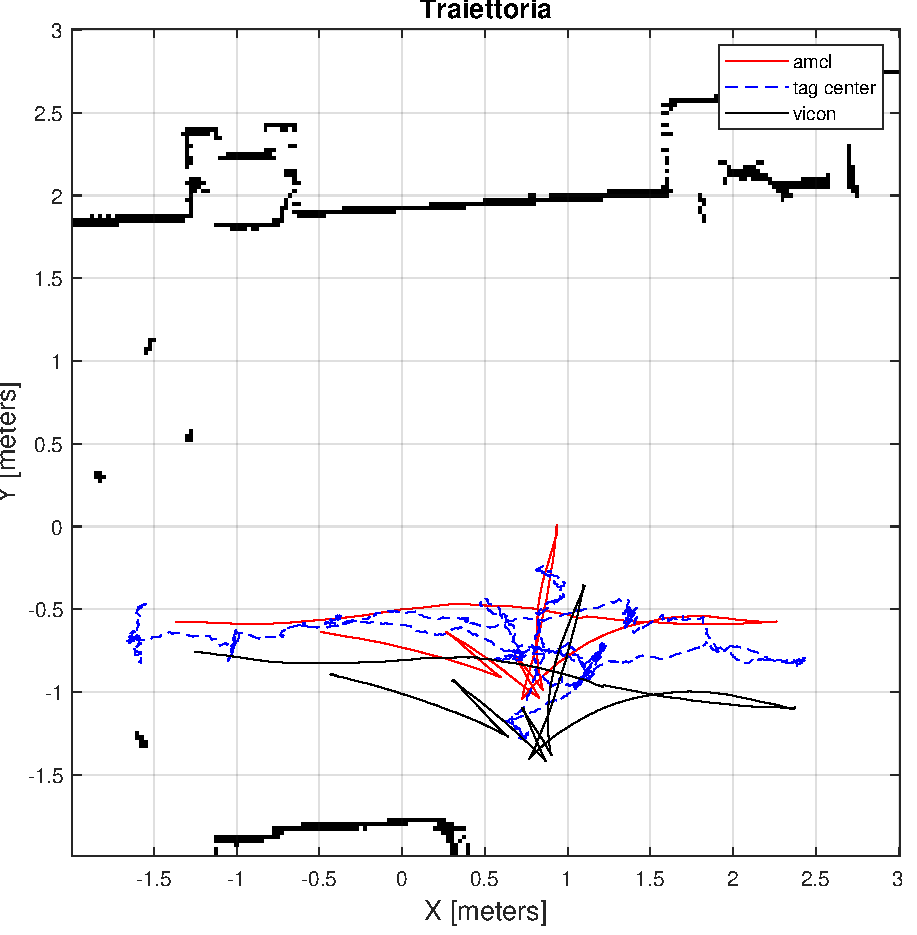
\includegraphics[height=.4\textheight]{grafici_stanzavolo_vicon/figure1.pdf}
	\caption{Traiettorie registrate con Vicon, UWB e navigazione con AMCL}
	\label{fig: traiettorie_vicon_charlie}
\end{figure}

\begin{figure}[] 
	\centering    
	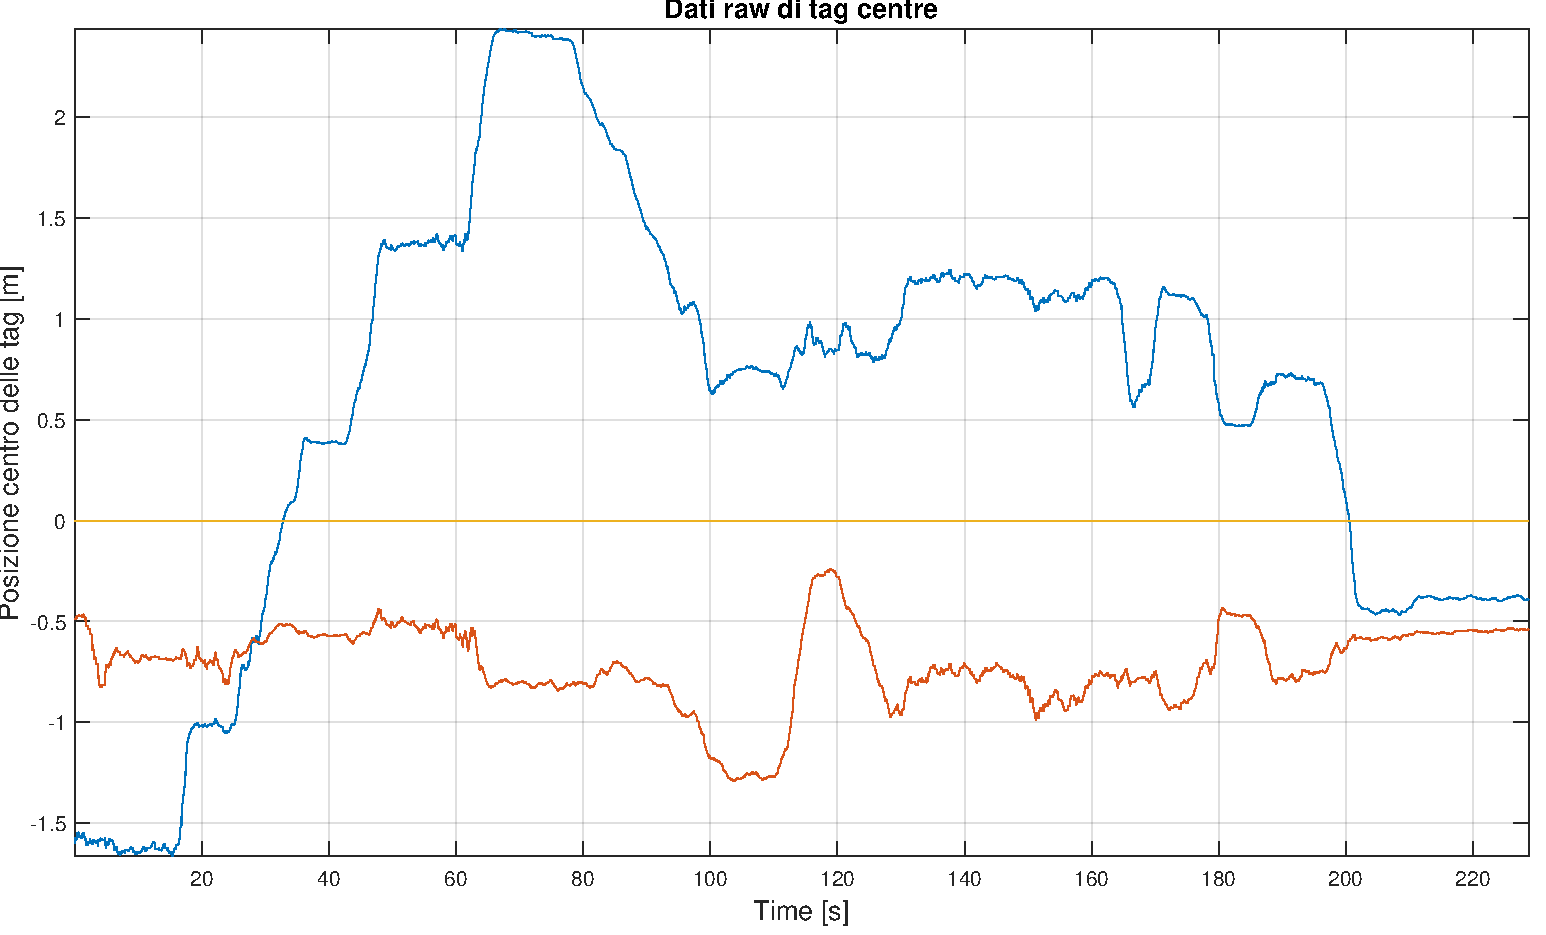
\includegraphics[height=.3\textheight]{grafici_stanzavolo_vicon/figure5.pdf}
	\caption{Coordinate lungo l'asse x in map frame registrate con Vicon, UWB e navigazione con AMCL}
	\label{fig: asse_x_vicon_charlie}
\end{figure}

\begin{figure}[] 
	\centering    
	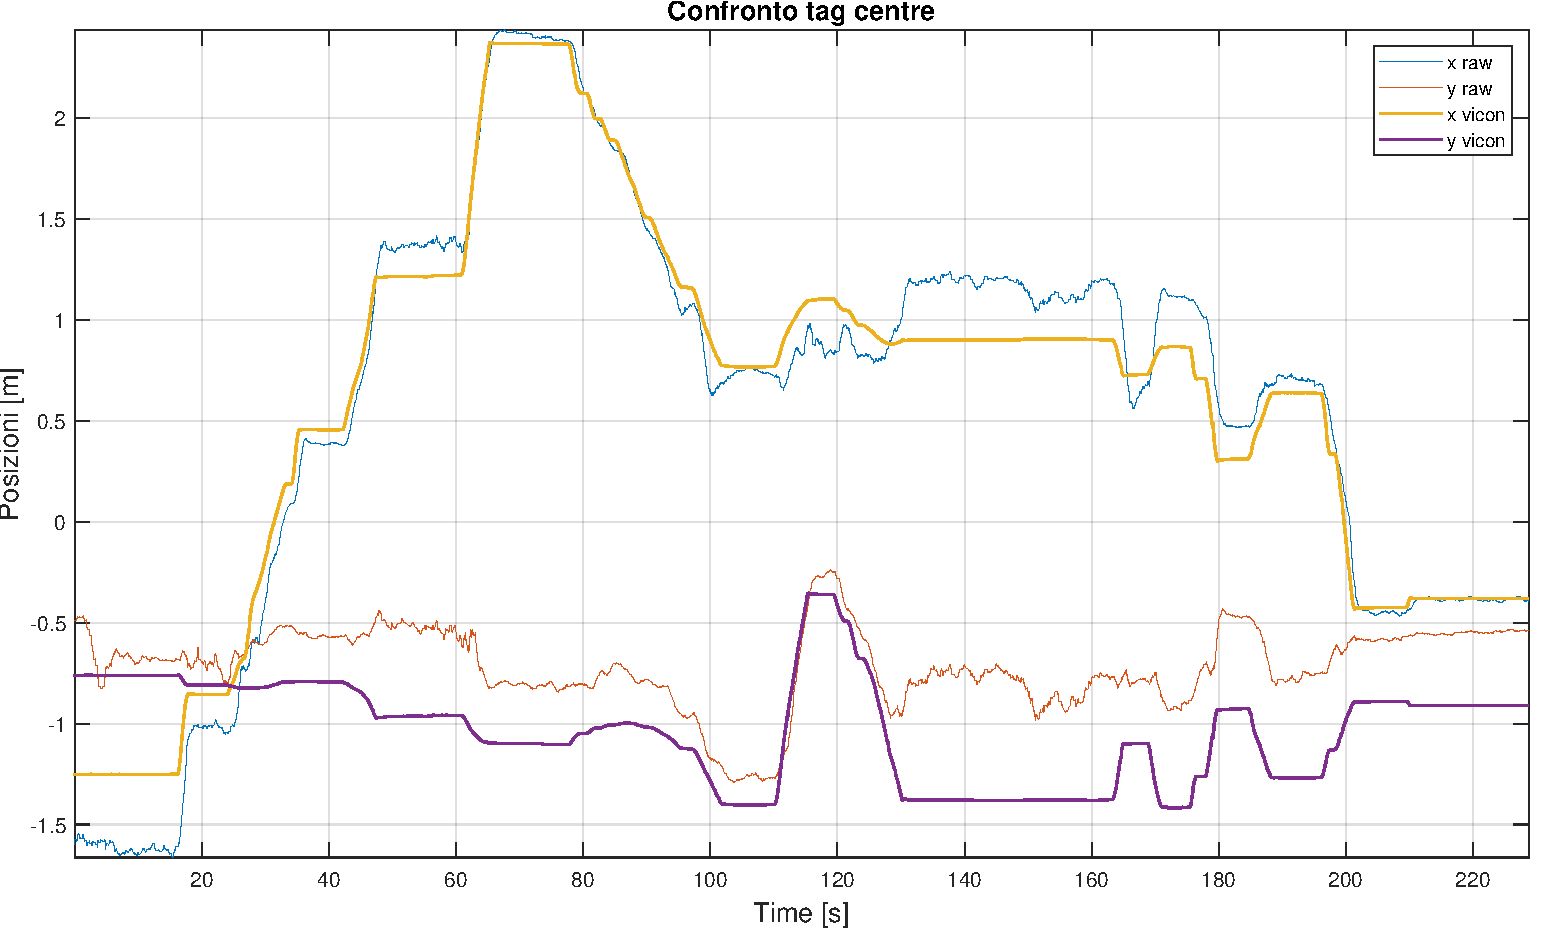
\includegraphics[height=.3\textheight]{grafici_stanzavolo_vicon/figure6.pdf}
	\caption{Coordinate lungo l'asse y in map frame registrate con Vicon, UWB e navigazione con AMCL}
	\label{fig: asse_y_vicon_charlie}
\end{figure}

\begin{figure}[] 
	\centering    
	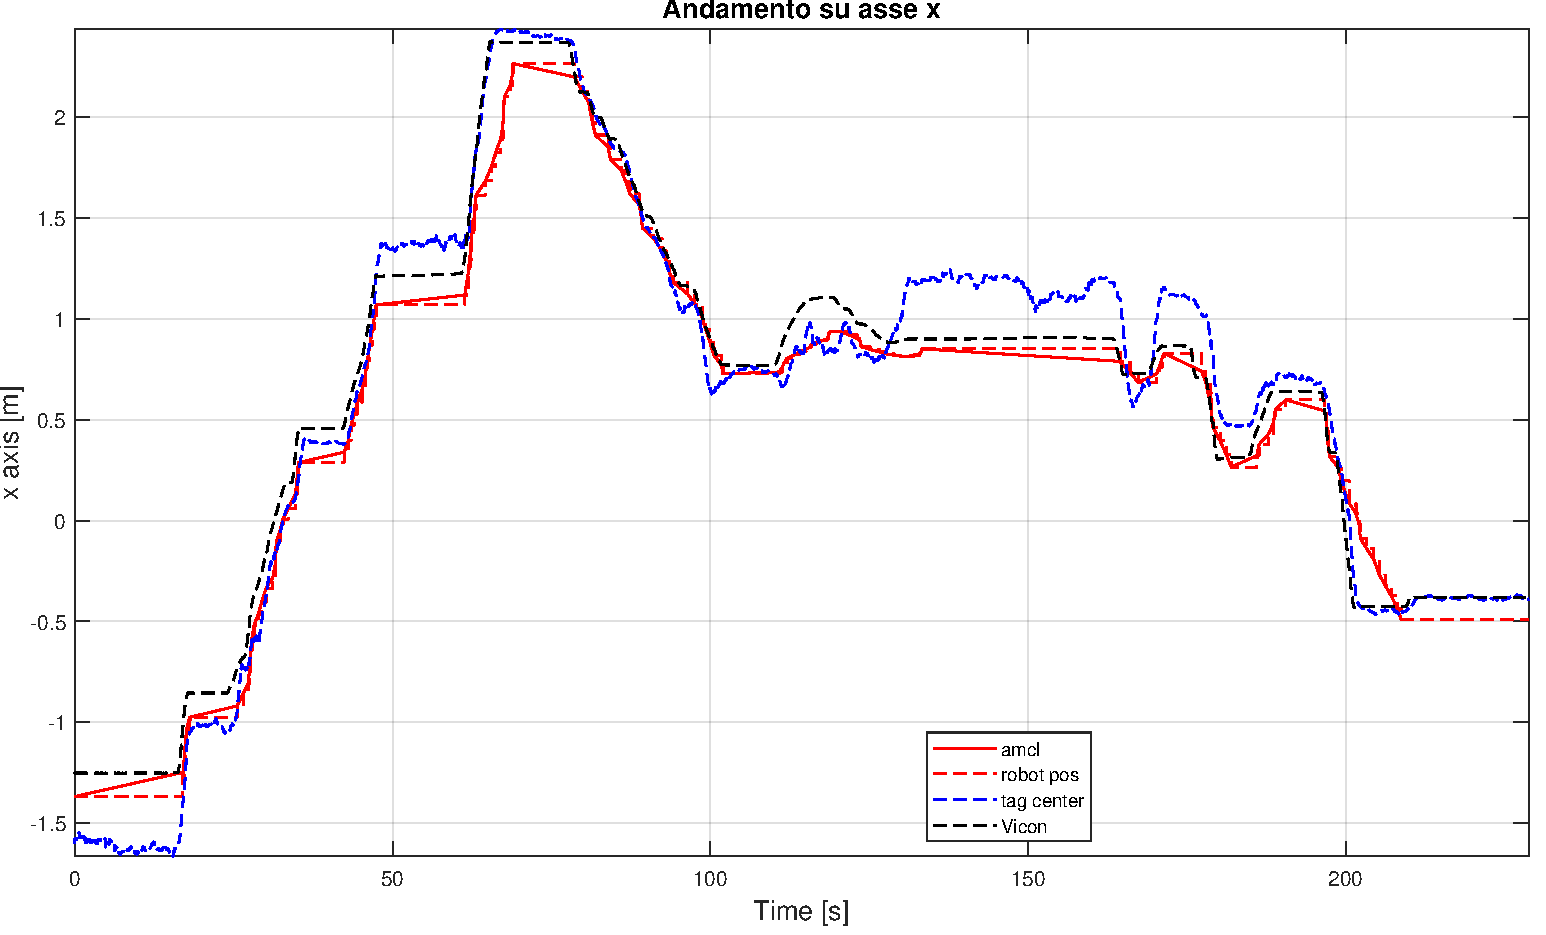
\includegraphics[height=.3\textheight]{grafici_stanzavolo_vicon/figure2.pdf}
	\caption{Heading in map frame registrate con Vicon, UWB e navigazione con AMCL}
	\label{fig: heading_vicon_charlie}
\end{figure}

\begin{figure}[] 
	\centering    
	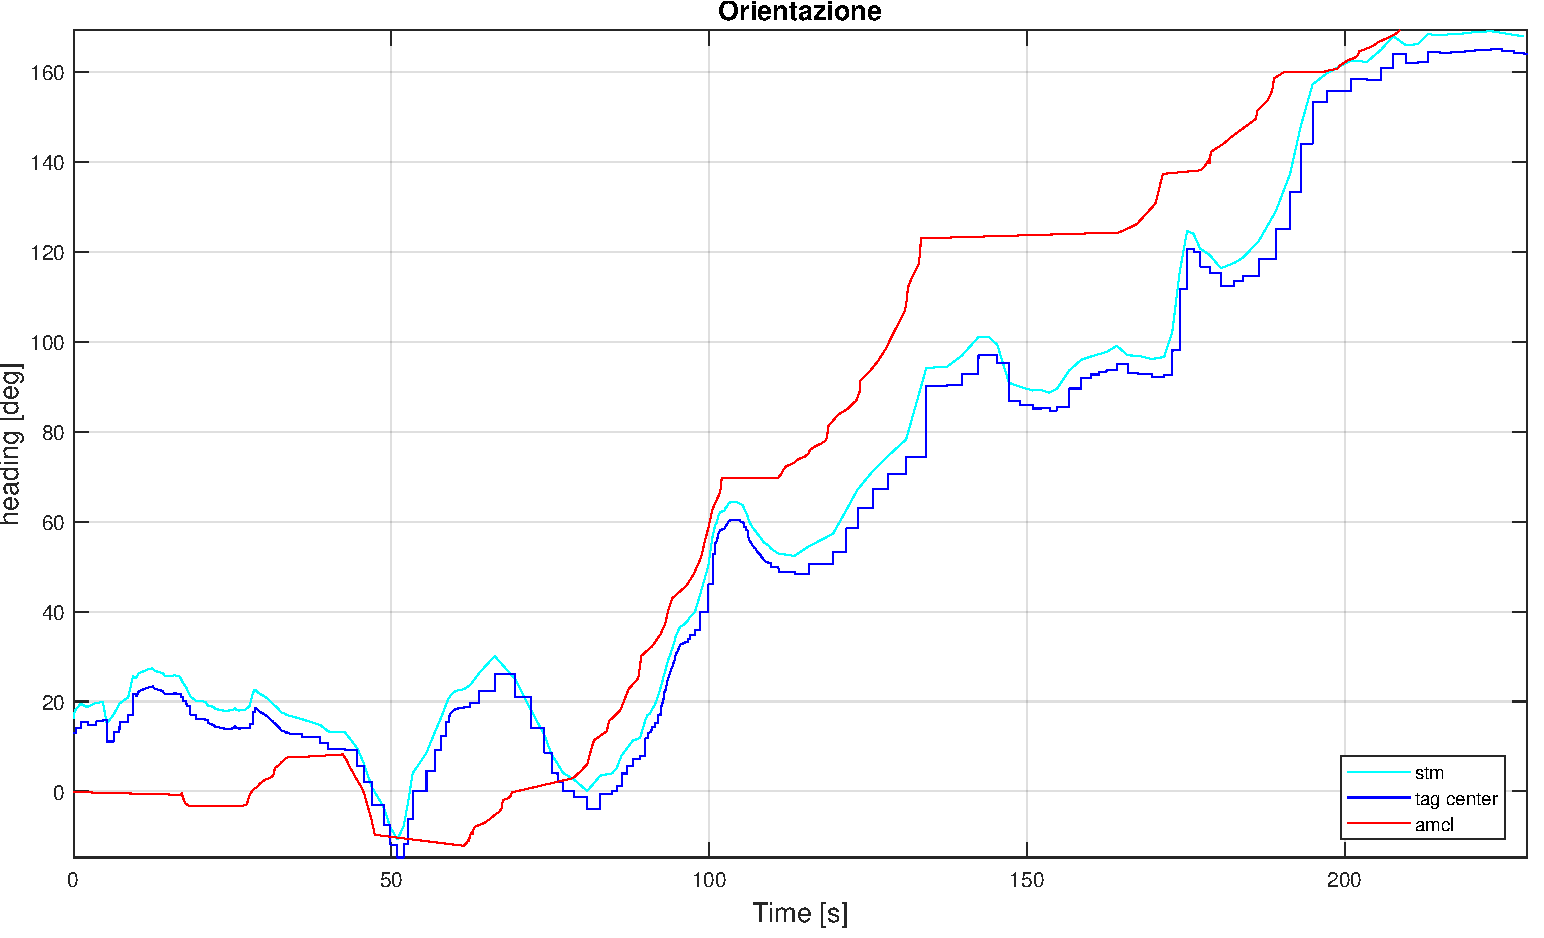
\includegraphics[height=.3\textheight]{grafici_stanzavolo_vicon/figure4.pdf}
	\caption{Coordinate lungo x e y in map frame registrate con Vicon, UWB e navigazione con AMCL}
	\label{fig: assixy_vicon_charlie}
\end{figure}

\begin{figure}[] 
	\centering    
	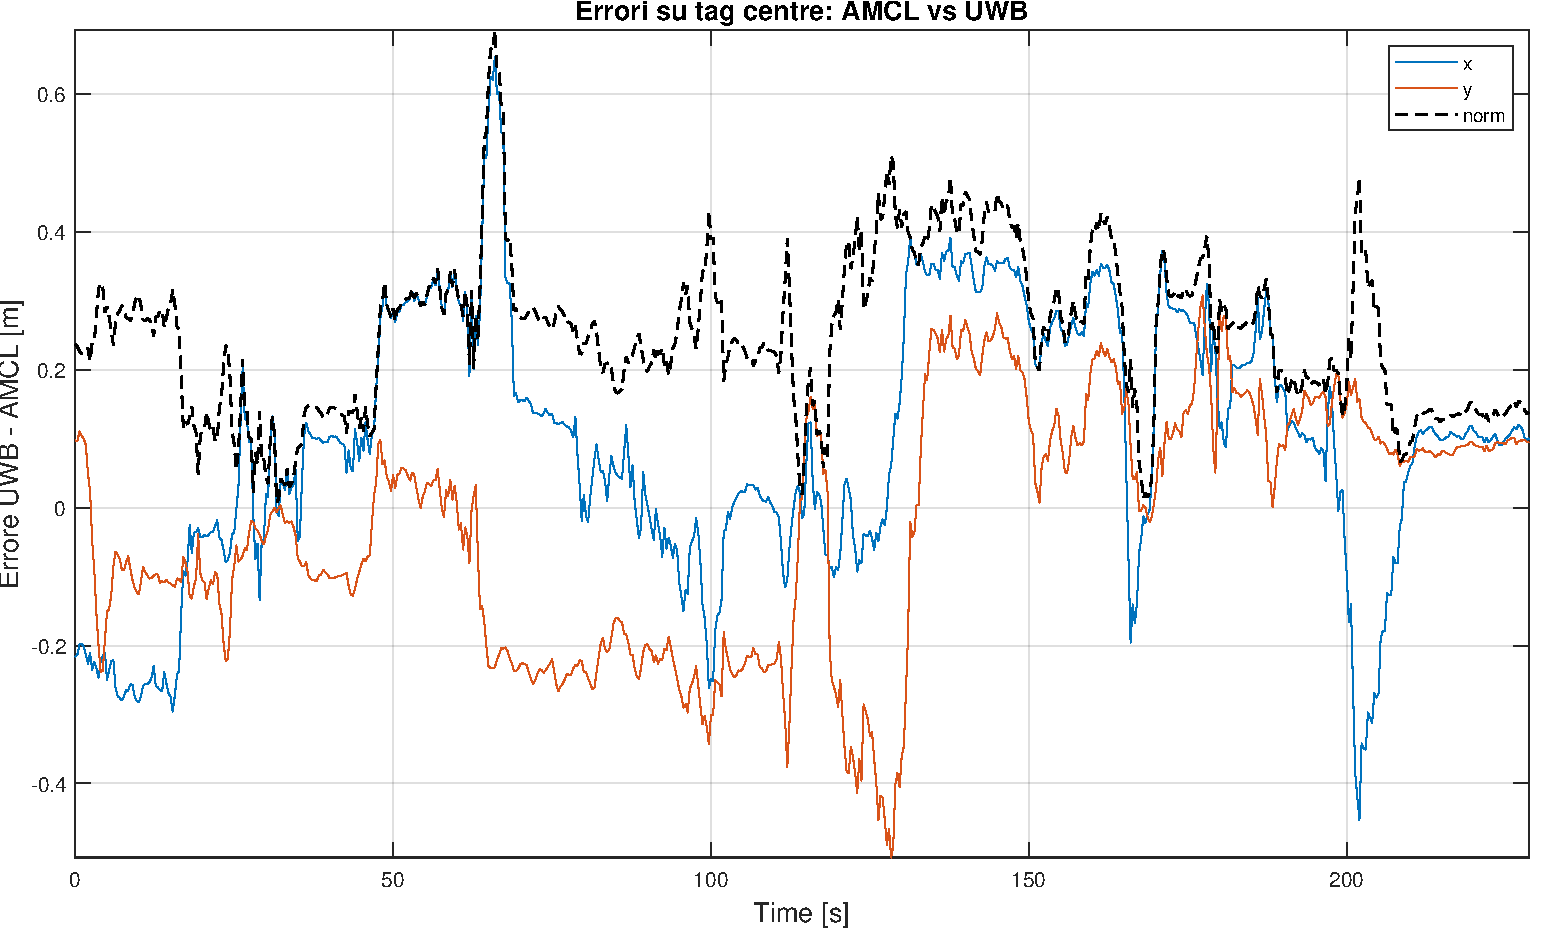
\includegraphics[height=.3\textheight]{grafici_stanzavolo_vicon/figure12.pdf}
	\caption{Errore tra posizione data da navigazione con AMCL e UWB}
	\label{fig: amcluwb_err_vicon_charlie}
\end{figure}

\begin{figure}[] 
	\centering    
	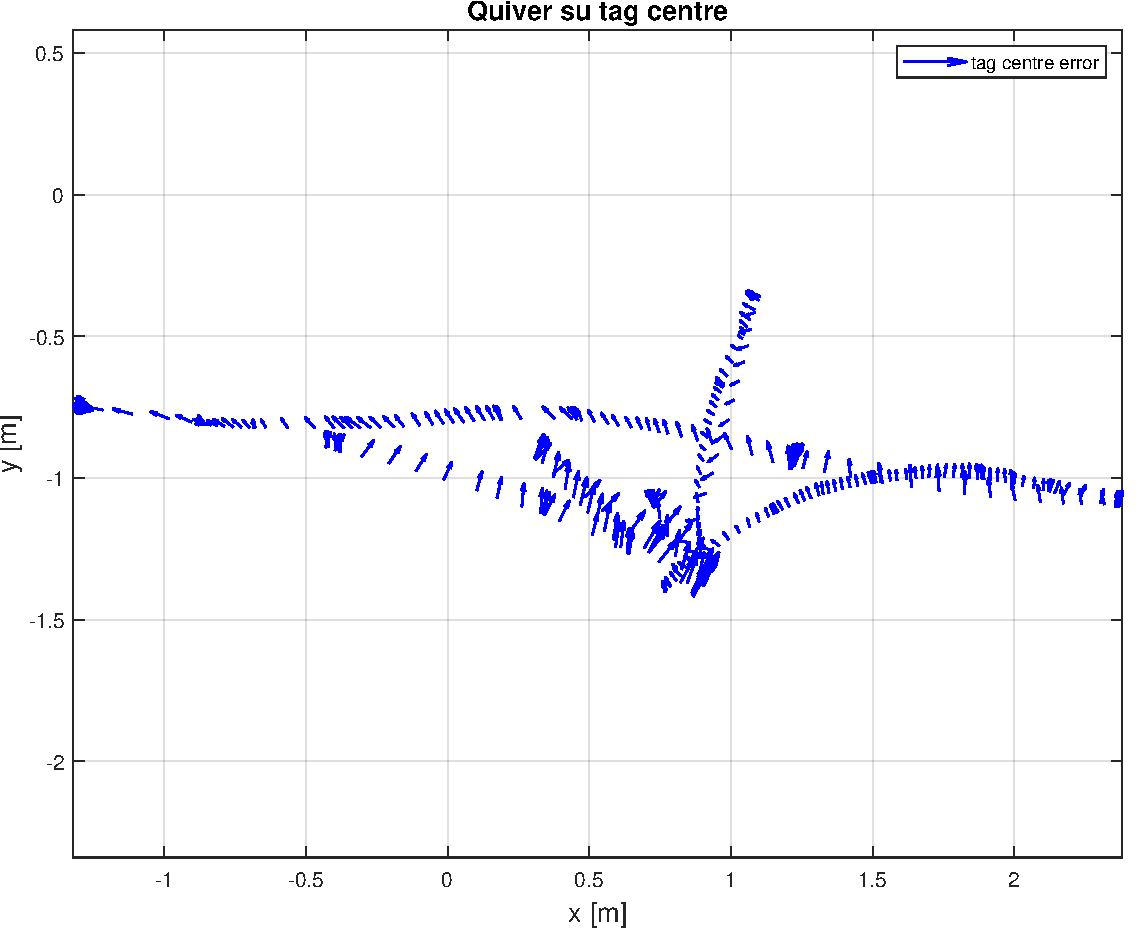
\includegraphics[height=.3\textheight]{grafici_stanzavolo_vicon/figure11.pdf}
	\caption{Errore tra posizione data da navigazione con AMCL e Vicon (ground truth)}
	\label{fig: amclvic_err_vicon_charlie}
\end{figure}

\begin{figure}[] 
	\centering    
	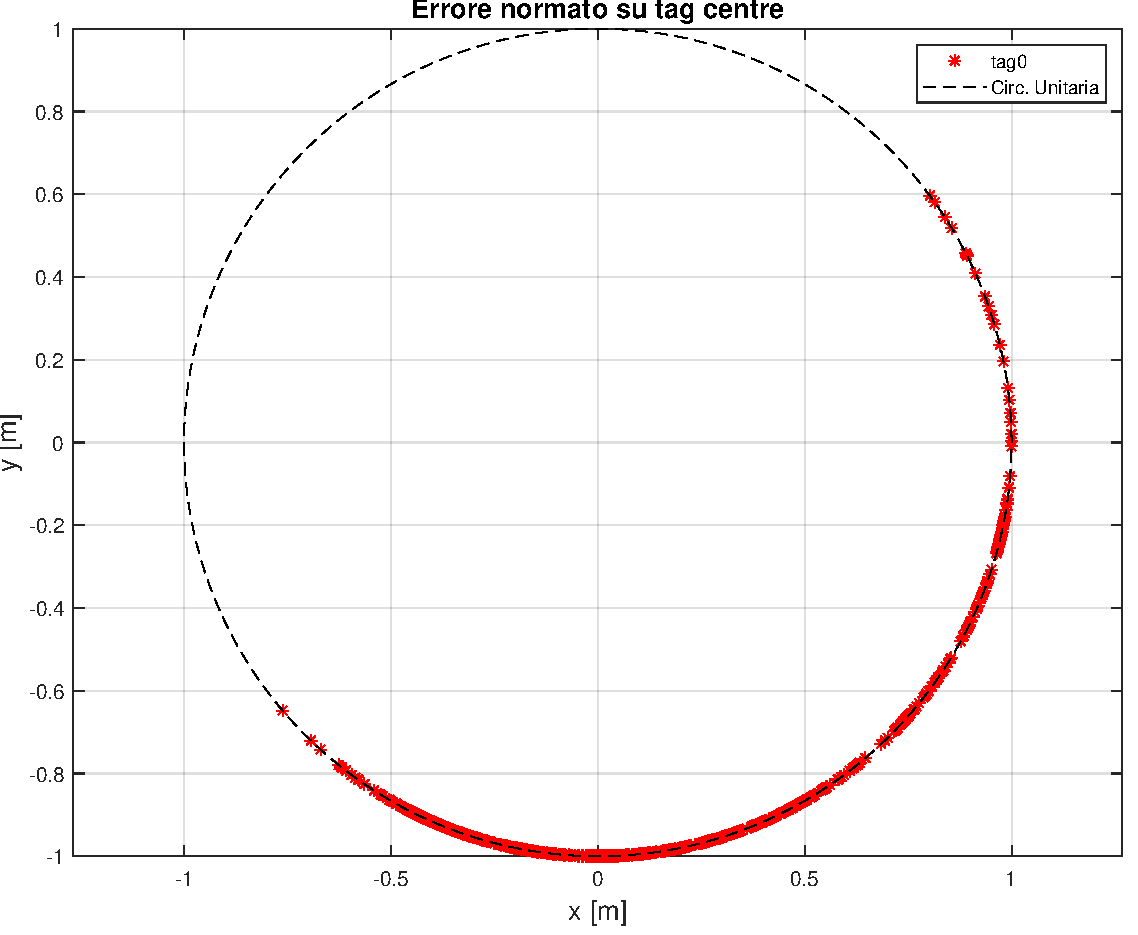
\includegraphics[height=.3\textheight]{grafici_stanzavolo_vicon/figure10.pdf}
	\caption{Errore tra posizione data da UWB e Vicon (ground truth)}
	\label{fig: uwbvic_err_vicon_charlie}
\end{figure}

\begin{figure}[] 
	\centering    
	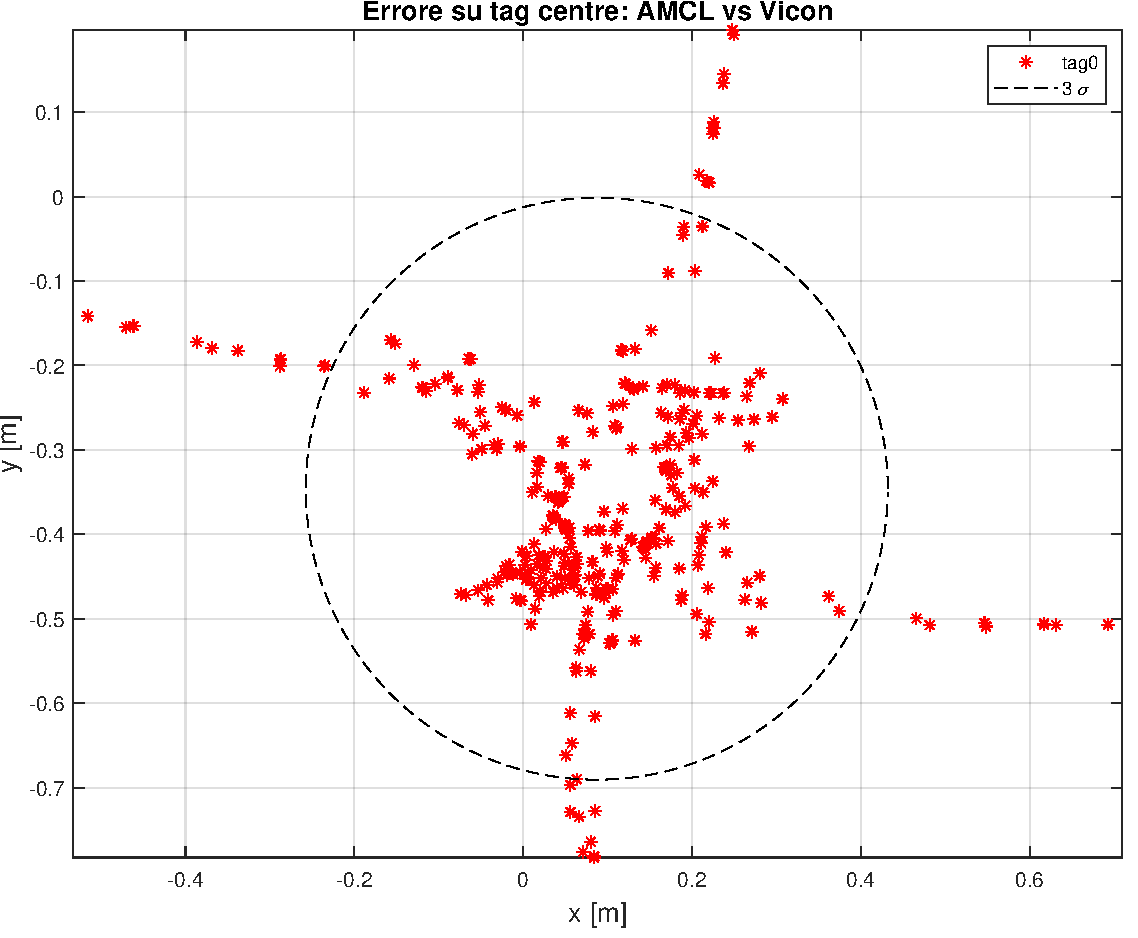
\includegraphics[height=.3\textheight]{grafici_stanzavolo_vicon/figure19.pdf}
	\caption{Distribuzione dell'errore tra posizione data da AMCL e dal Vicon (ground truth) }
	\label{fig: err_amclvic_sphere_vicon_charlie}
\end{figure}

\begin{figure}[] 
	\centering    
	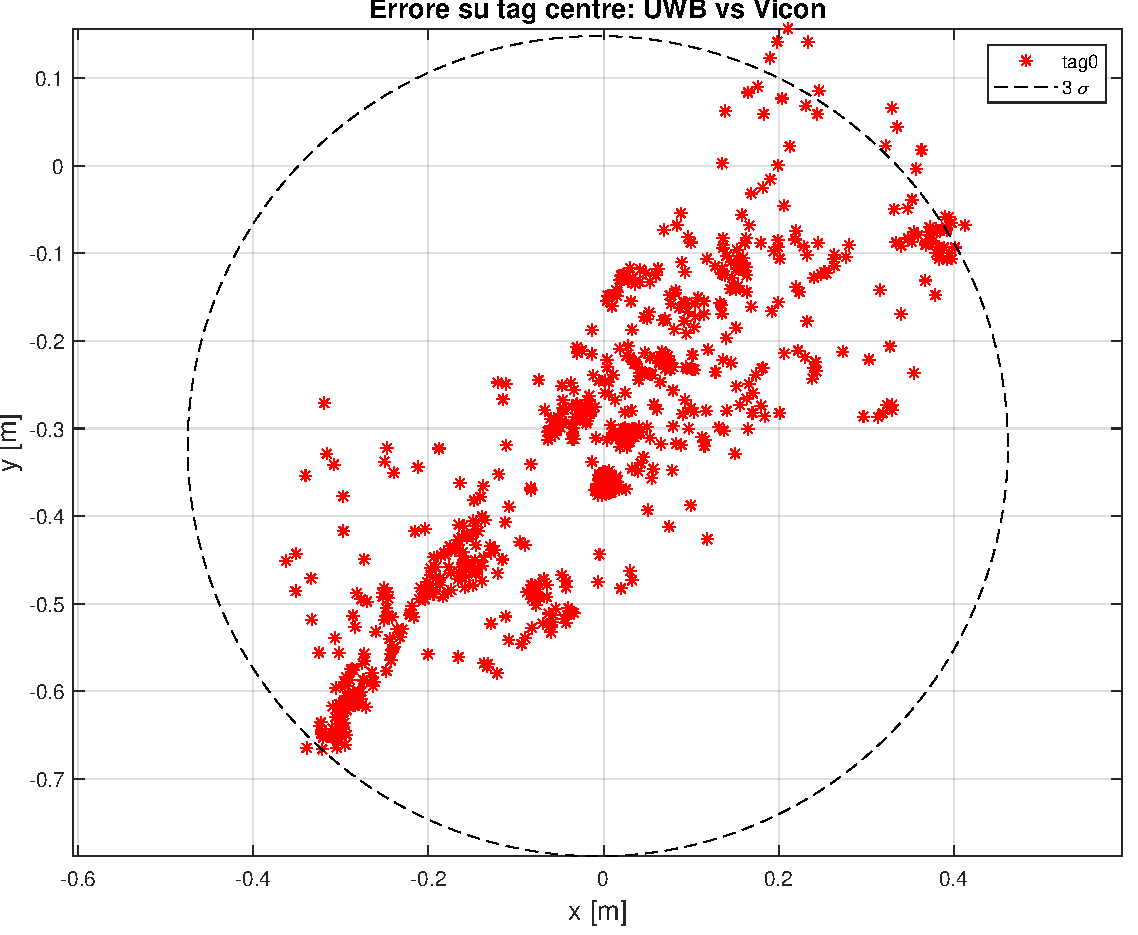
\includegraphics[height=.3\textheight]{grafici_stanzavolo_vicon/figure13.pdf}
	\caption{Distribuzione dell'errore tra posizione data da UWB e dal Vicon (ground truth)}
	\label{fig: err_uwbvic_sphere_vicon_charlie}
\end{figure}

%\begin{figure}[] 
%	\centering    
%	\includegraphics[height=.2\textheight]{grafici_stanzavolo_vicon/figure14_charlie_vic.pdf}
%	\caption{err uwbamcl sphere vicon charlie}
%	\label{fig: err_uwbamcl_sphere_vicon_charlie}
%\end{figure}

\begin{figure}[] 
	\centering    
	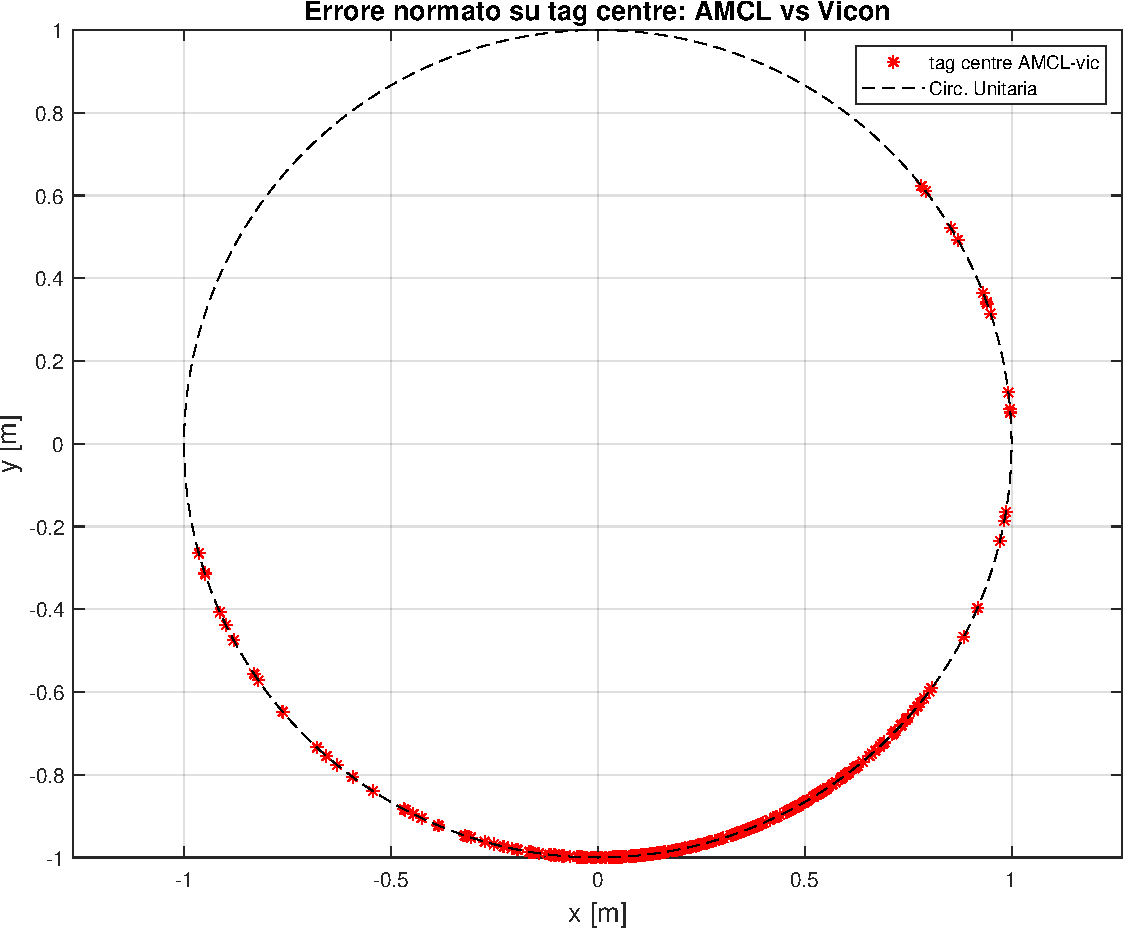
\includegraphics[height=.3\textheight]{grafici_stanzavolo_vicon/figure16.pdf}
	\caption{Distribuzione del versore errore tra la posizione data da AMCL e quella data dal Vicon su una circonferenza unitaria}
	\label{fig: err_norm_amclvic_sphere_vicon_charlie}
\end{figure}

\begin{figure}[] 
	\centering    
	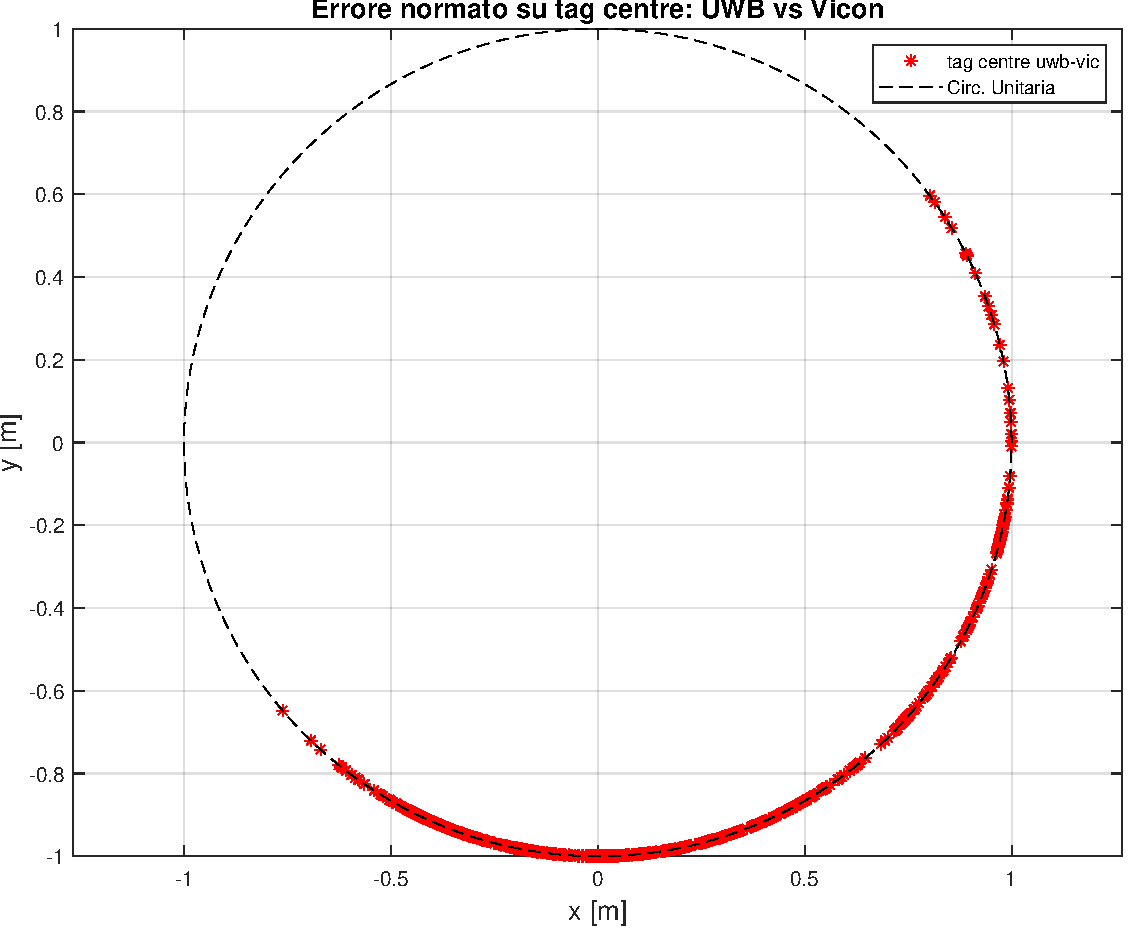
\includegraphics[height=.3\textheight]{grafici_stanzavolo_vicon/figure15.pdf}
	\caption{Distribuzione del versore errore tra la posizione data da UWB e quella data dal Vicon su una circonferenza unitaria}
	\label{fig: err_norm_uwbvic_sphere_vicon_charlie}
\end{figure}

\begin{figure}[] 
	\centering    
	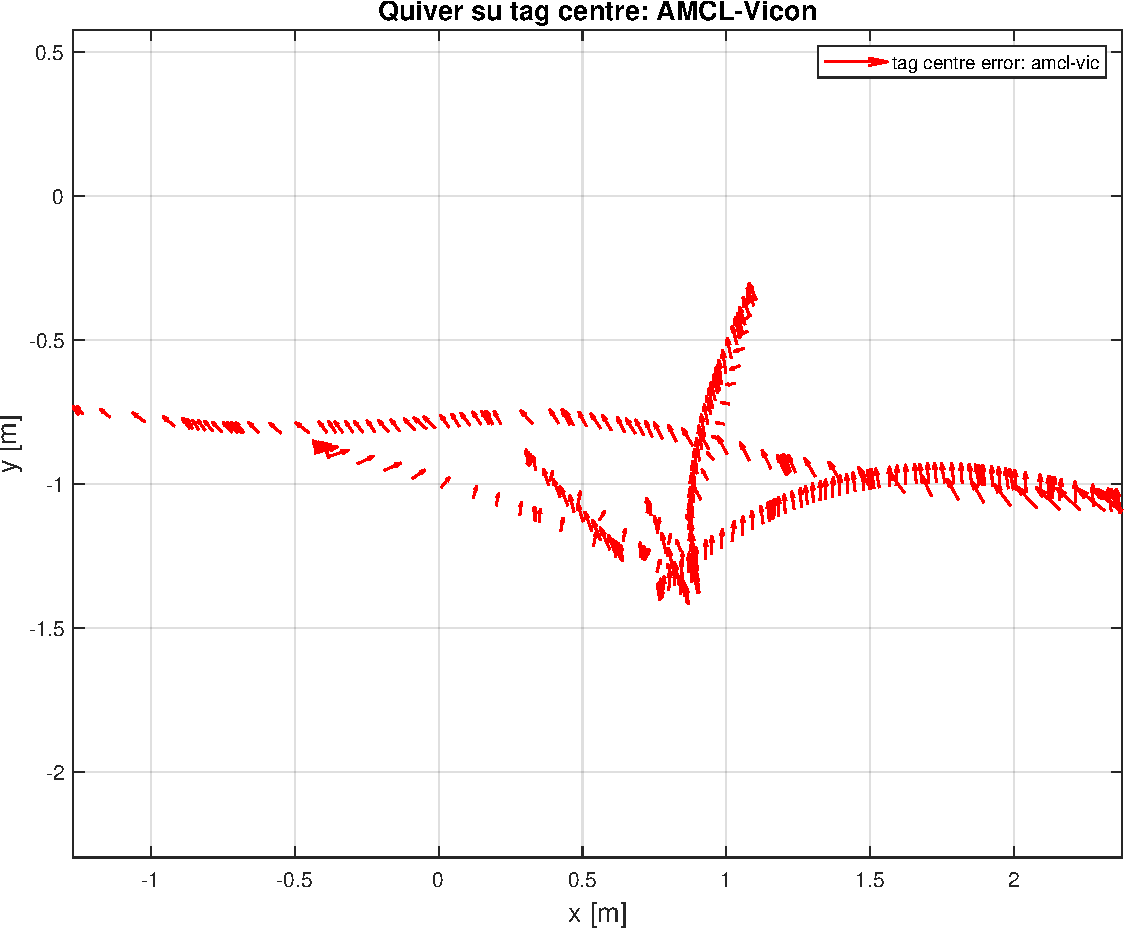
\includegraphics[height=.3\textheight]{grafici_stanzavolo_vicon/figure21.pdf}
	\caption{Distribuzione del vettore errore tra la posizione data da AMCL e quella data dal Vicon lungo la traiettoria}
	\label{fig: quiver_err_amclvic_vicon_charlie}
\end{figure}

\begin{figure}[] 
	\centering    
	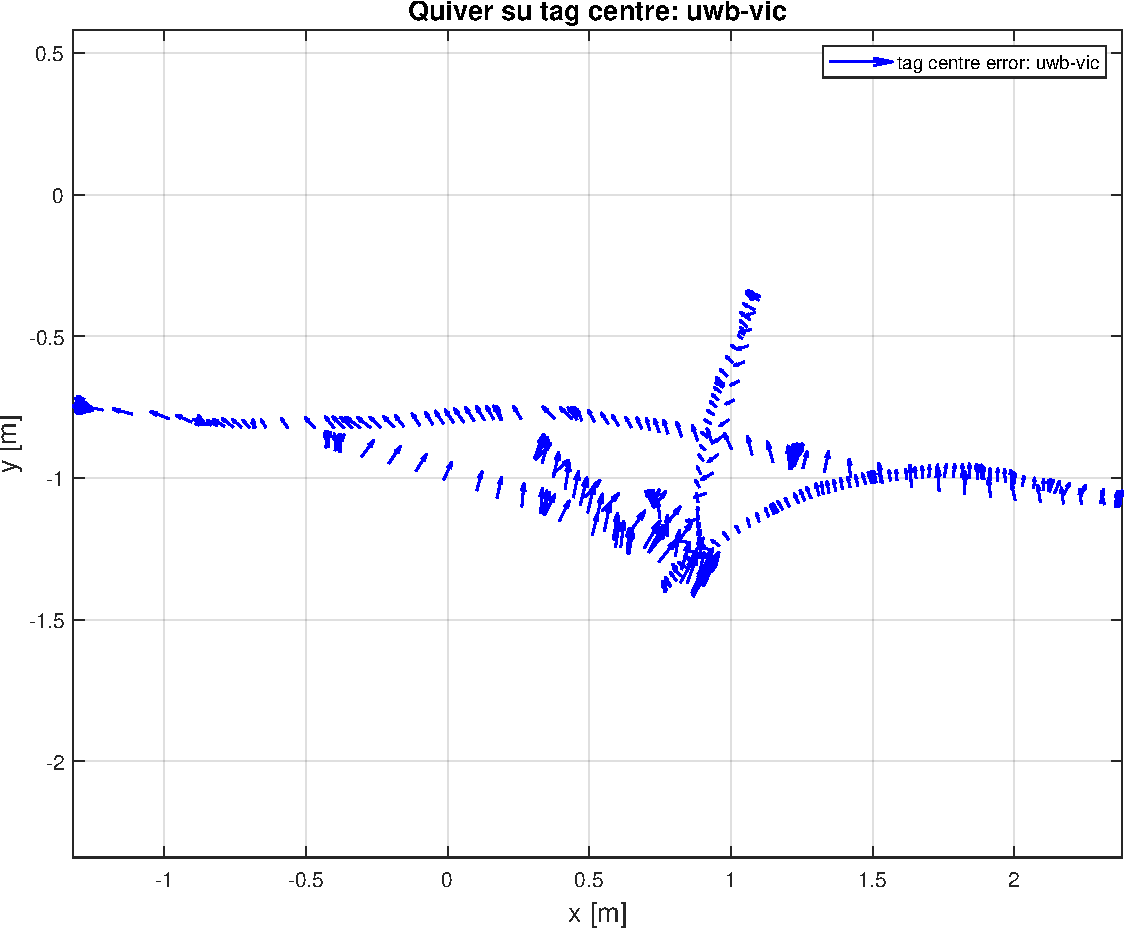
\includegraphics[height=.3\textheight]{grafici_stanzavolo_vicon/figure20.pdf}
	\caption{Distribuzione del vettore errore tra la posizione data da UWB e quella data dal Vicon lungo la traiettoria}
	\label{fig: quiver_err_uwbvic_vicon_charlie}
\end{figure}

\textbf{metti i quiver zoom}

Osservando i grafici relativi all'errore proiettato su una circonferenza unitaria, possiamo vedere che esiste una certa direzione 
preferenziale lungo la quale questo errore si presenta, sia per quanto riguarda il confronto tra la posizione in uscita dall'algoritmo AMCL e 
quella fornita dal sistema Vicon, vedere fig.~\ref{fig: err_norm_amclvic_sphere_vicon_charlie}, sia per quello tra quest'ultimo e la posizione data dal sistema Pozyx, come si nota in fig.~\ref{fig: err_norm_uwbvic_sphere_vicon_charlie}. 
Si può dedurre quindi la presenza di un errore sistematico, sia per quanto riguarda le misure delle ancore sia per l'algoritmo di navigazione con AMCL. Avendo però perso l'informazione relativa all'istante in cui si ha un determinato errore, non siamo in grado basandoci solo su questi grafici di tratte conclusioni esaustive sul fenomeno. Per questo motivo, abbiamo successivamente analizzato qual è l'errore, come vettore di errore, tra la posizione di AMCL o UWB rispetto a quella del nostro ground truth, vale a dire il sistema Vicon: questo è stato mostrato lungo tutta la traiettoria compiuta, in modo da poter indagare l'esistenza di errori sistematici che si verificano ogni volta che Charlie ripassa nello stesso punto della mappa ad istanti diversi. 
Tale analisi è riportata rispettivamente in fig.~\ref{fig: quiver_err_amclvic_vicon_charlie} e in fig.~\ref{fig: quiver_err_uwbvic_vicon_charlie}, dove osserviamo i vettori errore distribuiti lungo l'intera traiettoria. Da questi risultati possiamo osservare due fenomeni: il primo è direzione preferenziale, punti passaggi multipli hanno errore sistematico?

\textbf{IMPOSTA SU MATLAB LA ROBA PER LE ANALISI
	FAI ANALISI QUA}



\subsection{Navigazione con AMCL nel cortile}
Per l'esperimento nel cortile interno, torniamo a riferirci a \ref{sez: Guida breve all'esperimento}, dove troviamo passo passo tutti i comandi dati per 
l'esecuzione di una prova standard come questa.
La particolarità di questo esperimento, nonché il suo obiettivo, è quello di testare il sistema in ambiente outdoor, per di più caratterizzato da molti disturbi 
alla presenza nell'ambiente di grandi strutture metalliche e finestre. Non trascurabile, inoltre, una salita ampia, dove il lidar può trovarsi in difficoltà.

Prima di procedere con l'esperimento, è stata svolta una valutazione su come posizionare le ancore in base all'ambiente stesso: per aumentare la distanza tra di 
esse, abbiamo deciso di porre due ancore nella zona in salita, assicurandoci però di equilibrare i sostegni affinché non fossero anch'essi inclinati con l'utilizzo 
di un rialzo in uno dei piedini del sostegno stesso. Le prime tre ancore sono state quindi regolate affinché le tre schede (le ancore propriamente dette) si 
trovassero allo stesso livello in linea d'aria (alla stessa quota). Per la quarta ancora, è stata posta vicino all'origine, come nelle configurazioni precedenti, 
perché in seguito a molte prove abbiamo riscontrato essere la configurazione che restituisce migliori autocalibrazioni. In merito a ciò, una volta scelte le 
posizioni definitive delle ancore, abbiamo proceduto proprio con l'effettuare l'autocalibrazione. Anche le misure con il metro a nastro sono state effettuate, 
affinché avessimo un termine di confronto attendibile, anche se soggetto a errori. Da qua l'esperimento procede standard, come in \ref{sez: Guida breve all'esperimento}. 
Dopo la costruzione della nuova mappa, si lancia il file \verb|localization.launch| e si registra il tutto in una bag.

\textbf{FAI ANALISI QUA, bozza sotto}


prima prova: inizio stai praticamente fermo, si vede che a un certo punto abbiamo un offset tra valore di UWB e valore di AMCL. Offset rimane durante il moto successivo, che 
è lento qua. Vediamo diversi fix di posa, legati al fatto che il filtro AMCL rimane indietro rispetto all'esecuzione real time. 

seconda prova: andiamo più veloci. vediamo che AMCL si perde completamente perché non ha assolutamente tempo di eseguire l'algoritmo in tempo entro il nuovo aggiornamento di 
posa, quindi rimane costantemente indietro e passa da un fix di posa al successivo. Il fix di posa stesso è molto lento, infatti nel mentre non c'è modo di capire
che sta eseguendo un fix di posa e l'utente, continuando a muoversi con Charlie accumula errore grande in termini di differenza tra l'ultima posizione nota a AMCL e UWB attuale.
Anche l'orientazione rimane indietro, sia con AMCL sia con UWB. Con UWB, ciò succede perché viene utilizzata l'informazione di \verb|orientation|, dove si calcola l'orientazione come \verb|atan_2| tra le posizioni delle due tag: il tutto viene filtrato con una media mobile, che introduce un ritardo.

terza prova: come la seconda ma andando più lenti, si vede comunque un ritardo da parte di AMCL nonostante si vada molto piano.

queste analisi ci portano a concludere che sarebbe opportuno cambiare algo di navigazione in quanto i fix di posa e l'esecuzione di AMCL prendono troppo tempo e non permettono una applicazione fluida online anche a velocità irrisorie: esisterà sempre una velocità per la quale si accumula un ritardo di AMCL che porta a un fix di posa. Ad ogni modo, anche settando in modo diverso la distanza entro cui lanciare il fix di posa, si avrebbe lo stesso problema.

%%%%%%%%%%%%%%%%%%%%%%%%%%%%%%%%%%%%%%%%%%%%%%%%%%%%%%%%%%%%%%%%%%%%%%%%%%%%%%%%%%%%%%%%%%%%%%%%%%%%%%
\newpage
\section{Guida breve all'esperimento}
\label{sez: Guida breve all'esperimento}
In questa sezione è riportata, sommariamente, la procedura da eseguire per lanciare un esperimento completo. Per una guida dettagliata, riferirsi a 
sez.~\ref{sez:L'esperimento}. 

Prima di tutto, è necessario disporre le ancore come descritto in sez.~\ref{sez:Sistema Pozyx}, come si può vedere in fig.~\ref{fig: disposizione ancore}. 
Assicurarsi di aver impostato correttamente le impostazioni WiFi (sez.~\ref{sez: primo collegamento a raspberry}) e di avere il PC e la Raspberry connessi 
alla stessa rete WiFi.


Connettersi poi in \textbf{ssh} alla Raspberry dal PC digitando, da terminale del PC e con password \texttt{robot}, il seguente comando:
\begin{lstlisting}[style=bashPC]
	ssh -X -C pi@raspberrypi.local		# avvia ssh
\end{lstlisting}

Per l'\textbf{autocalibrazione} (necessaria ogni volta che viene riposizionato il sistema di ancore) lanciare 
dalla cartella \texttt{home} (da terminale della Raspberry):
\begin{lstlisting}[style=bash]
	python3 ~/charlie_autocalibration/autocalibration_ransac.py
\end{lstlisting}
infine, rispondere ``y'' per salvare i risultati nella memoria flash delle ancore (necessario per avere informazioni corrette sulle loro posizioni, vedere 
sez.~\ref{sez:Sistema Pozyx}).

Adesso è necessario avviare il \textbf{posizionamento} delle tag pozyx e la comunicazione \textbf{seriale} con Icaro (suggeriamo di utilizzare più terminali 
con \href{https://terminator-gtk3.readthedocs.io/en/latest/}{terminator}):
\begin{lstlisting}[style=bash]
	roslaunch charlie_launch start_uwb.launch		# avvia uwb
	roslaunch charlie_launch start_serial.launch	# avvia seriale con stm
\end{lstlisting}

\subsection{Nuova Mappa}
\label{sez: nuova mappa}
Una nuova mappa è necessaria quando si cambia posizionamento alle ancore o banalmente si cambia luogo. Consigliamo di muovere Charlie attraverso il radiocomando 
in questa fase, per averne un maggiore controllo, soprattutto in termini di limitarne la velocità di avanzamento, che in questa fase di acquisizione della mappa 
è bene che sia molto bassa.
\begin{lstlisting}[style=bash]
	roslaunch charlie_launch save_map_origin.launch		# con Charlie fermo!
	roslaunch charlie_launch new_map.launch 			# muovere Charlie lentamente
\end{lstlisting}

Una volta soddisfatti del risultato, salvare la mappa all'interno di una cartella dedicata, detta qua \verb|maps| attraverso i comandi:
\begin{lstlisting}[style=bash]
	cd charlie_ws/maps
	rosrun map_server map_saver -f NOME_MAPPA
\end{lstlisting}

\subsection{Localizzazione}
Prima di procedere, è necessario sostituire il nome della mappa che si vuole utilizzare all'interno del file:

\verb|/home/pi/charlie_ws/src/charlie_launch/launch/localization.launch|:

\begin{lstlisting}[style=xml, firstnumber=14]
	<arg name="file_NUM" default="NOME_MAPPA" />
	<node name="map_server" pkg="map_server" type="map_server" args="$(arg path)$(arg file_NUM).yaml"/>
\end{lstlisting}

Quindi, si può adesso lanciare il file appena modificato con il comando standard per eseguire file \verb|.launch|:
\begin{lstlisting}[style=bash]
	roslaunch charlie_launch localization.launch
\end{lstlisting}

All'interno dello stesso file è predisposta anche la possibilità di visualizzare rviz attraverso la connessione ssh con il ``Compressed X11 Forwarding '', 
scommentando la riga corrispondente di rviz. Questa opzione è però molto sconsigliata da noi, in quanto rende la visione poco reattiva. Per ovviare a questo 
problema, dopo aver configurato pc e raspberry come descritto in sez.~\ref{sez: Ros master/slave}, è possibile lanciare direttamente dal terminale del pc il comando:

\begin{lstlisting}[style=bashPC]
	roslaunch charlie_remote rviz_remote.launch
\end{lstlisting}
Così da aprire rviz da pc, ma sfruttando il master su raspberry.
In questo momento l'esperimento è iniziato!

\subsection{Waypoints}
\`E possibile indicare una posa-goal tramite il comando \texttt{2DNavgoal} direttamente da rviz (tenere premuto per assegnare l'orientazione).
Per attivare i motori e permettere al robot di spostarsi, pubblicare il seguente messaggio sul topic \verb|start\_and\_stop|:

\begin{lstlisting}[style=bash]
	rostopic pub /start_and_stop std_msgs/Float64 "data: 1.0"
\end{lstlisting}
Si consiglia di farlo una volta dato il comando del waypoint da raggiungere con rviz.
Per fermarli, similmente, è sufficiente pubblicare il messaggio complementare, sempre sul topic \verb|start\_and\_stop|:

\begin{lstlisting}[style=bash]
	rostopic pub /start_and_stop std_msgs/Float64 "data: 0.0"
\end{lstlisting}

\subsection{Sistema Vicon}
Ovviamente, per poter utilizzare il sistema Vicon è necessario trovarsi nella stanza del volo del DII. 
Per quanto concerne l'installazione, rifarsi a sez.~\ref{sez:Sistema Vicon}. 
Una volta che il sistema è in funzione, avviare l'applicazione ``Vicon Tracker 3.7.0 x64'' e selezionare nella lista oggetti: \texttt{Charlie} e 
\texttt{Active Wand v2 (Origin Tracking)}. 
Connettere poi il computer fisso, a sua volta attaccato fisicamente al sistema Vicon (che sarà il server Vicon), alla stessa rete in cui abbiamo già
raspberry e pc. In seguito, modificare nel file di lancio \texttt{charlie\_remote/launch/vicon\_charlie.launch} l'ip del server Vicon nella seguente riga:
\begin{lstlisting}[style=xml, firstnumber=6]
	<arg name="server" default="IP_SERVER"/>
\end{lstlisting}

Per avviare i dialoghi tra ros e il sistema Vicon, eseguire da pc il file di lancio \verb|vicon_charlie.launch|con il comando:
\begin{lstlisting}[style=bashPC]
	roslaunch charlie_remote vicon_charlie.launch
\end{lstlisting}

Salvare poi la trasformazione tra vicon e uwb (all'utente sarà richiesto di posizionare la wand, in successione, sulle verie ancore):
\begin{lstlisting}[style=bashPC]
	rosrun charlie_remote vicon2uwb_tf.py
\end{lstlisting}

e, infine, lanciare il nodo che pubblica la posizione di Charlie in frame map:
\begin{lstlisting}[style=bashPC]
	rosrun charlie_remote charlie_vicon2map.py
\end{lstlisting}


\subsection{Rosbag}
Per registrare i dati attraverso una rosbag suggeriamo di non sottoscriversi a tutti i topic, in quanto verrebbero salvati molti elementi non necessari 
al nostro esperimento. Si consiglia quindi di lanciare il seguente comando da pc (dopo essersi spostati nella cartella desiderata nella quale salvare i 
file \verb|.bag|), contenente la selezione da noi fatta in merito ai topic ai quali sottoscriversi per ottenere tutti e soli i dati di nostro interesse:
\begin{lstlisting}[style=bashPC]
	rosbag record /clock /initialpose /map /orientation /particlecloud /robot_pose /rosout /rosout_agg /scan /tag_center /tf /amcl_pose /charlie_vicon_map -O NOME_BAG.bag
\end{lstlisting}

Per eseguire i topic necessari ad AMCL, prima riconfigurare il file:

\verb|../charlie_remote/launch/exec_bag.launch| con i file e il path che si vogliono utilizzare e quindi lanciare da pc:
\begin{lstlisting}[style=bashPC]
	roslaunch charlie_remote exec_bag.launch
\end{lstlisting}
e da raspberry (modificando il nome della mappa da utilizzare all'interno del file di lancio \verb|localization_bag.launch|):
\begin{lstlisting}[style=bash]
	roslaunch charlie_launch localization_bag.launch
\end{lstlisting}

%%%%%%%%%%%%%%%%%%%%%%%%%%%%%%%%%%%%%%%%%%%%%%%%%%%%%%%%%%%%%%%%%%%%%%%%%%


% Bibliography
\newpage
\bibliography{biblio}


\end{document}